\documentclass[twocolumn]{article}
\usepackage[top=1.1in, left=0.85in, right=0.85in]{geometry}

\usepackage{amsmath}
\usepackage{amssymb}
\usepackage{code}
\usepackage{graphicx}
\usepackage{fancyvrb}
\usepackage{url}
\usepackage{textcomp}
% \usepackage{inlinebib}

\pagestyle{empty}

\newcommand\comment[1]{}
\newcommand\parameteralert[1]{
  \begin{quotation}
  \noindent {\bf Parameter Alert!} #1
  \end{quotation}
}

\newcommand\st{$^{\mathrm{st}}$}
\newcommand\nd{$^{\mathrm{nd}}$}
\newcommand\rd{$^{\mathrm{rd}}$}
\renewcommand\th{$^{\mathrm{th}}$}
\newcommand\tm{$^{\mbox{\tiny \textsc{tm}}}$}

% nice fractions
\newcommand\sfrac[2]{{}\,$^{#1}$\!/{}\!$_{#2}$}

\newcommand\citef[1]{\addtocounter{footnote}{1}\footnotetext{\cite{#1}}\ensuremath{^{\mbox{\footnotesize [\thefootnote]}}}}

% \usepackage{ulem}
% go back to italics for emphasis, though
% \normalem

\begin{document} 

\title{The First Level of Super Mario Bros.~is Easy with
       Lexicographic Orderings and Time Travel
       {\normalsize \ldots after that it gets a little tricky.}}
\author{Dr.~Tom~Murphy~VII~Ph.D.\thanks{
Copyright \copyright\ 2013 the Regents of the Wikiplia
Foundation. Appears in SIGBOVIK 2013 with the reluctant sigh of the
Association for Computational Heresy; {\em IEEEEEE!} press,
Verlag-Verlag volume no.~0x40-2A.
CHF 0.00}
}

\renewcommand\>{$>$}
\newcommand\<{$<$}

\date{1 April 2013}

\maketitle

\begin{abstract}
% XXX better abstract
This paper presents a simple, generic method for automating the play
of Nintendo Entertainment System games.
\end{abstract}

\vspace{1em}
{\noindent \small {\bf Keywords}:
  computational super mario brothers, memory inspection, lexicographic induction, networked entertainment systems, pit-jumping, ...

}

\section{Introduction}
The Nintendo Entertainment System is probably the best video game
console, citation {\it not} needed. Like many, I have spent thousands
of hours of my life playing NES games, including several complete
playthroughs of classics like Super Mario Bros., Bionic Commando,
Bubble Bobble, and other favorites. By the year 2013, home computers
have become many orders of magnitude faster and more capacious than
the NES hardware. This suggested to me that it may be time to automate
the playing of NES games, in order to save time.\footnote{Rather, to
  replace it with time spent programming.} In this paper I present a
generic technique for automating the playing of NES games. The
approach is practical on a single computer, and succeeds on several
games, such as Super Mario Bros.. The approach is amusingly elegant
and surprisingly effective, requires no detailed knowledge of the game
being played, and is capable of novel and impressive gameplay (for
example, bug exploitation). {\bf Disclaimer for SIGBOVIK audience:
  This work is 100\% real.}

On a scale from ``the title starts with Toward'' to ``Donald Knuth has
finally finished the 8\th\ volume on the subject,'' this work is a 3.
The purpose of this paper is mainly as a careful record of the current
status for repeatability and further development on this important
research subject. A short video version of this paper is available for
those that hate reading, at \verb+http://tom7.org/mario+, and is the
more fun way to consume the results. This page also contains
audiovisual material that makes this work more entertaining (for
example, its output) and source code.

The basic idea is to deduce an objective function from a short
recording of a player's inputs to the game. The objective function is
then used to guide search over possible inputs, using an emulator.
This allows the player's notion of progress to be generalized in order
to produce novel gameplay. A design goal is that the objective
function be amusingly elegant (not at all smart, fancy, or customized
to the game) in order to demonstrate that the game is reducible to
such a simple objective. The search needs to be game-agnostic and
practical, but since the space is exponential
($256^{n}$)\cite{GeneralizedSuper}, we need to be smart here.

The objective function, the algorithm to deduce it, the search
strategy, and its implementation are all interesting and will be
discussed in that order. I then discuss the results of using the
approach to automate several NES games. To set the stage, I begin with
a description of the NES hardware and emulation of it.

\subsection{The NES hardware and emulation}
The NES is based around an 8-bit processor running at 1.79~MHz, the
Ricoh 2A03. 8 bits is really small. You can see them all right here:
00001111. It's no coincidence that each controller also has 8 buttons:
Up, Down, Left, Right, Select, Start, B and A. It has only 2048 bytes
of general purpose RAM. (There is also some special purpose RAM for
graphics, which we ignore in this work.) 2048 bytes is really small.
You can see them all in Figure~\ref{fig:bytes2048}. As a result, NES
programs are written to use memory efficiently and straightforwardly;
usually there are fixed memory locations used for all the critical
game facts like the player's health, number of lives, coordinates on
the screen, and so on. For example, in Super Mario Bros., the single
byte at location \verb+0x757+ contains the number of lives the player
has. The location \verb+0x75F+ contains the current world, and
\verb+0x760+ the current level. The NES outputs 60.0988 frames per
second, which we will just call 60 in this paper.

% (32kB of ROM is addressable at a time, and most games used bank
% switching to access hundreds of kilobytes of game included in the
% cartridge.)

There are a number of emulators for NES. These work by simulating the
NES hardware, for example with a 2048-byte array for its memory, and
simulating the steps of its 2A03 processor on some ROM, and hooking a
keyboard or joystick into the 8 bits of input. (There are of course
many details to work out! But in essence emulation is just that.) This
process is completely deterministic, so it is possible to record the
sequence of inputs (the inputs can only be read once per video frame,
so this sequence is 60 bytes per second) and play them back and get
the same result. This also means that an input sequence can be
computed in non-real time, either much slower or much faster than a
NES would normally run. In this work we use the FCEUX\cite{FCEUX}
emulator, which is popular for its accuracy and advanced tools.

\begin{figure}[ht]
\begin{center}
% TODO: better if actual ram!

\includegraphics[width=0.75 \linewidth]{bytes2048}
\end{center}\vspace{-0.1in}
\caption{2048 bytes, a 64x32 image.}
\label{fig:bytes2048}
\end{figure}

\section{Objective function}

Bytes in memory (and sometimes 16- and 32-bit words) can contain
interesting game facts like the player's position in the level or
score. The central idea of this paper is to use (only) the value of
memory locations to deduce when the player is ``winning''. The things
that a human player perceives, like the video screen and sound
effects, are completely ignored. As an additional simplification, we
assume that winning always consists of a value {\it going up}---either
the position in the level getting larger, the score getting larger,
the number of lives, the world or level number getting bigger, and so
on.

This is actually a little bit too naive; for example, Mario's overall
progress through the game is represented by a pair. You start in World
{\tt 1-1} and the underground level that comes next is World {\tt 1-2}
(we'll call this $w=1$ and $\ell=2$). But after you discover the
princess is in another castle in World {\tt 1-4}, the next level is
{\tt 2-1}.\footnote{In case you never realized this, it is time to learn
  that the legendary ``Minus World'' of {\tt\, -1} is not actually a
  negative world, but World {\tt 36-1} being incorrectly rendered because
  there is no glyph for the 36\th\ digit. The trick used to get to the
  Minus World just happens to leave the value 36 in that memory
  location rather than initializing it to a useful value. The ROM does
  not contain data for world 36 so it just interprets garbage data as
  a description of the world.} This can't be represented as a single
byte going up (sometimes the second part $\ell$ goes down when we get
to a new first part $w$), but it can be represented as a lexicographic
order on the pair $\langle w, \ell \rangle$; that is, $\langle w_1,
\ell_1 \rangle < \langle w_2, \ell_2 \rangle$ if $w_1 = w_2$ and $\ell_1 <
\ell_2$, or if $w_1 < w_2$ no matter the values of $\ell_1$ and
$\ell_2$. This matches our intuitive idea and is also mathematically
nice. It also generalizes multi-byte encodings of things like your
score (which can be larger than 8 bits and so is often stored in 16 or
32), including both big-endian and little-endian
representations.\footnote{A possible additional simplification would
  be to just take lexicographic orderings over bits, which then
  generalizes to 8-bit bytes. This is probably too crazy, but just
  right now I am sort of feeling like maybe I should try it, though it
  may be the beer.}

More importantly, it allows the combination of semantically unrelated
bytes, like: $\langle$\!\!\!\! world, level, screen inside the world,
$x$ position on the screen \!\!$\rangle$ or $\langle$\!\!\!\! world,
lives, low byte of score \!\!$\rangle$. Many orderings may describe
gameplay. These orderings may be temporarily violated in normal play:
Although the score always goes up, Mario's $x$ position may
temporarily decrease if he needs to navigate around some
obstacle.\footnote{Note to self: Maybe we should give a much higher
  score to globally preserved objectives than to locally preserved
  ones. But that may presuppose that the input represents a whole
  playthrough?} So, to ``faithfully'' represent gameplay, we will
generate a set of lexicographic orderings on memory locations, with
the idea that they ``generally go up'' but not necessarily at every
step. These orderings will also have weights. The next section
describes how we take a sequence of player inputs and deduce the
orderings.

\subsection{Deriving the objective function} \label{sec:deriving}


\begin{figure}[h!tb]
\begin{center}
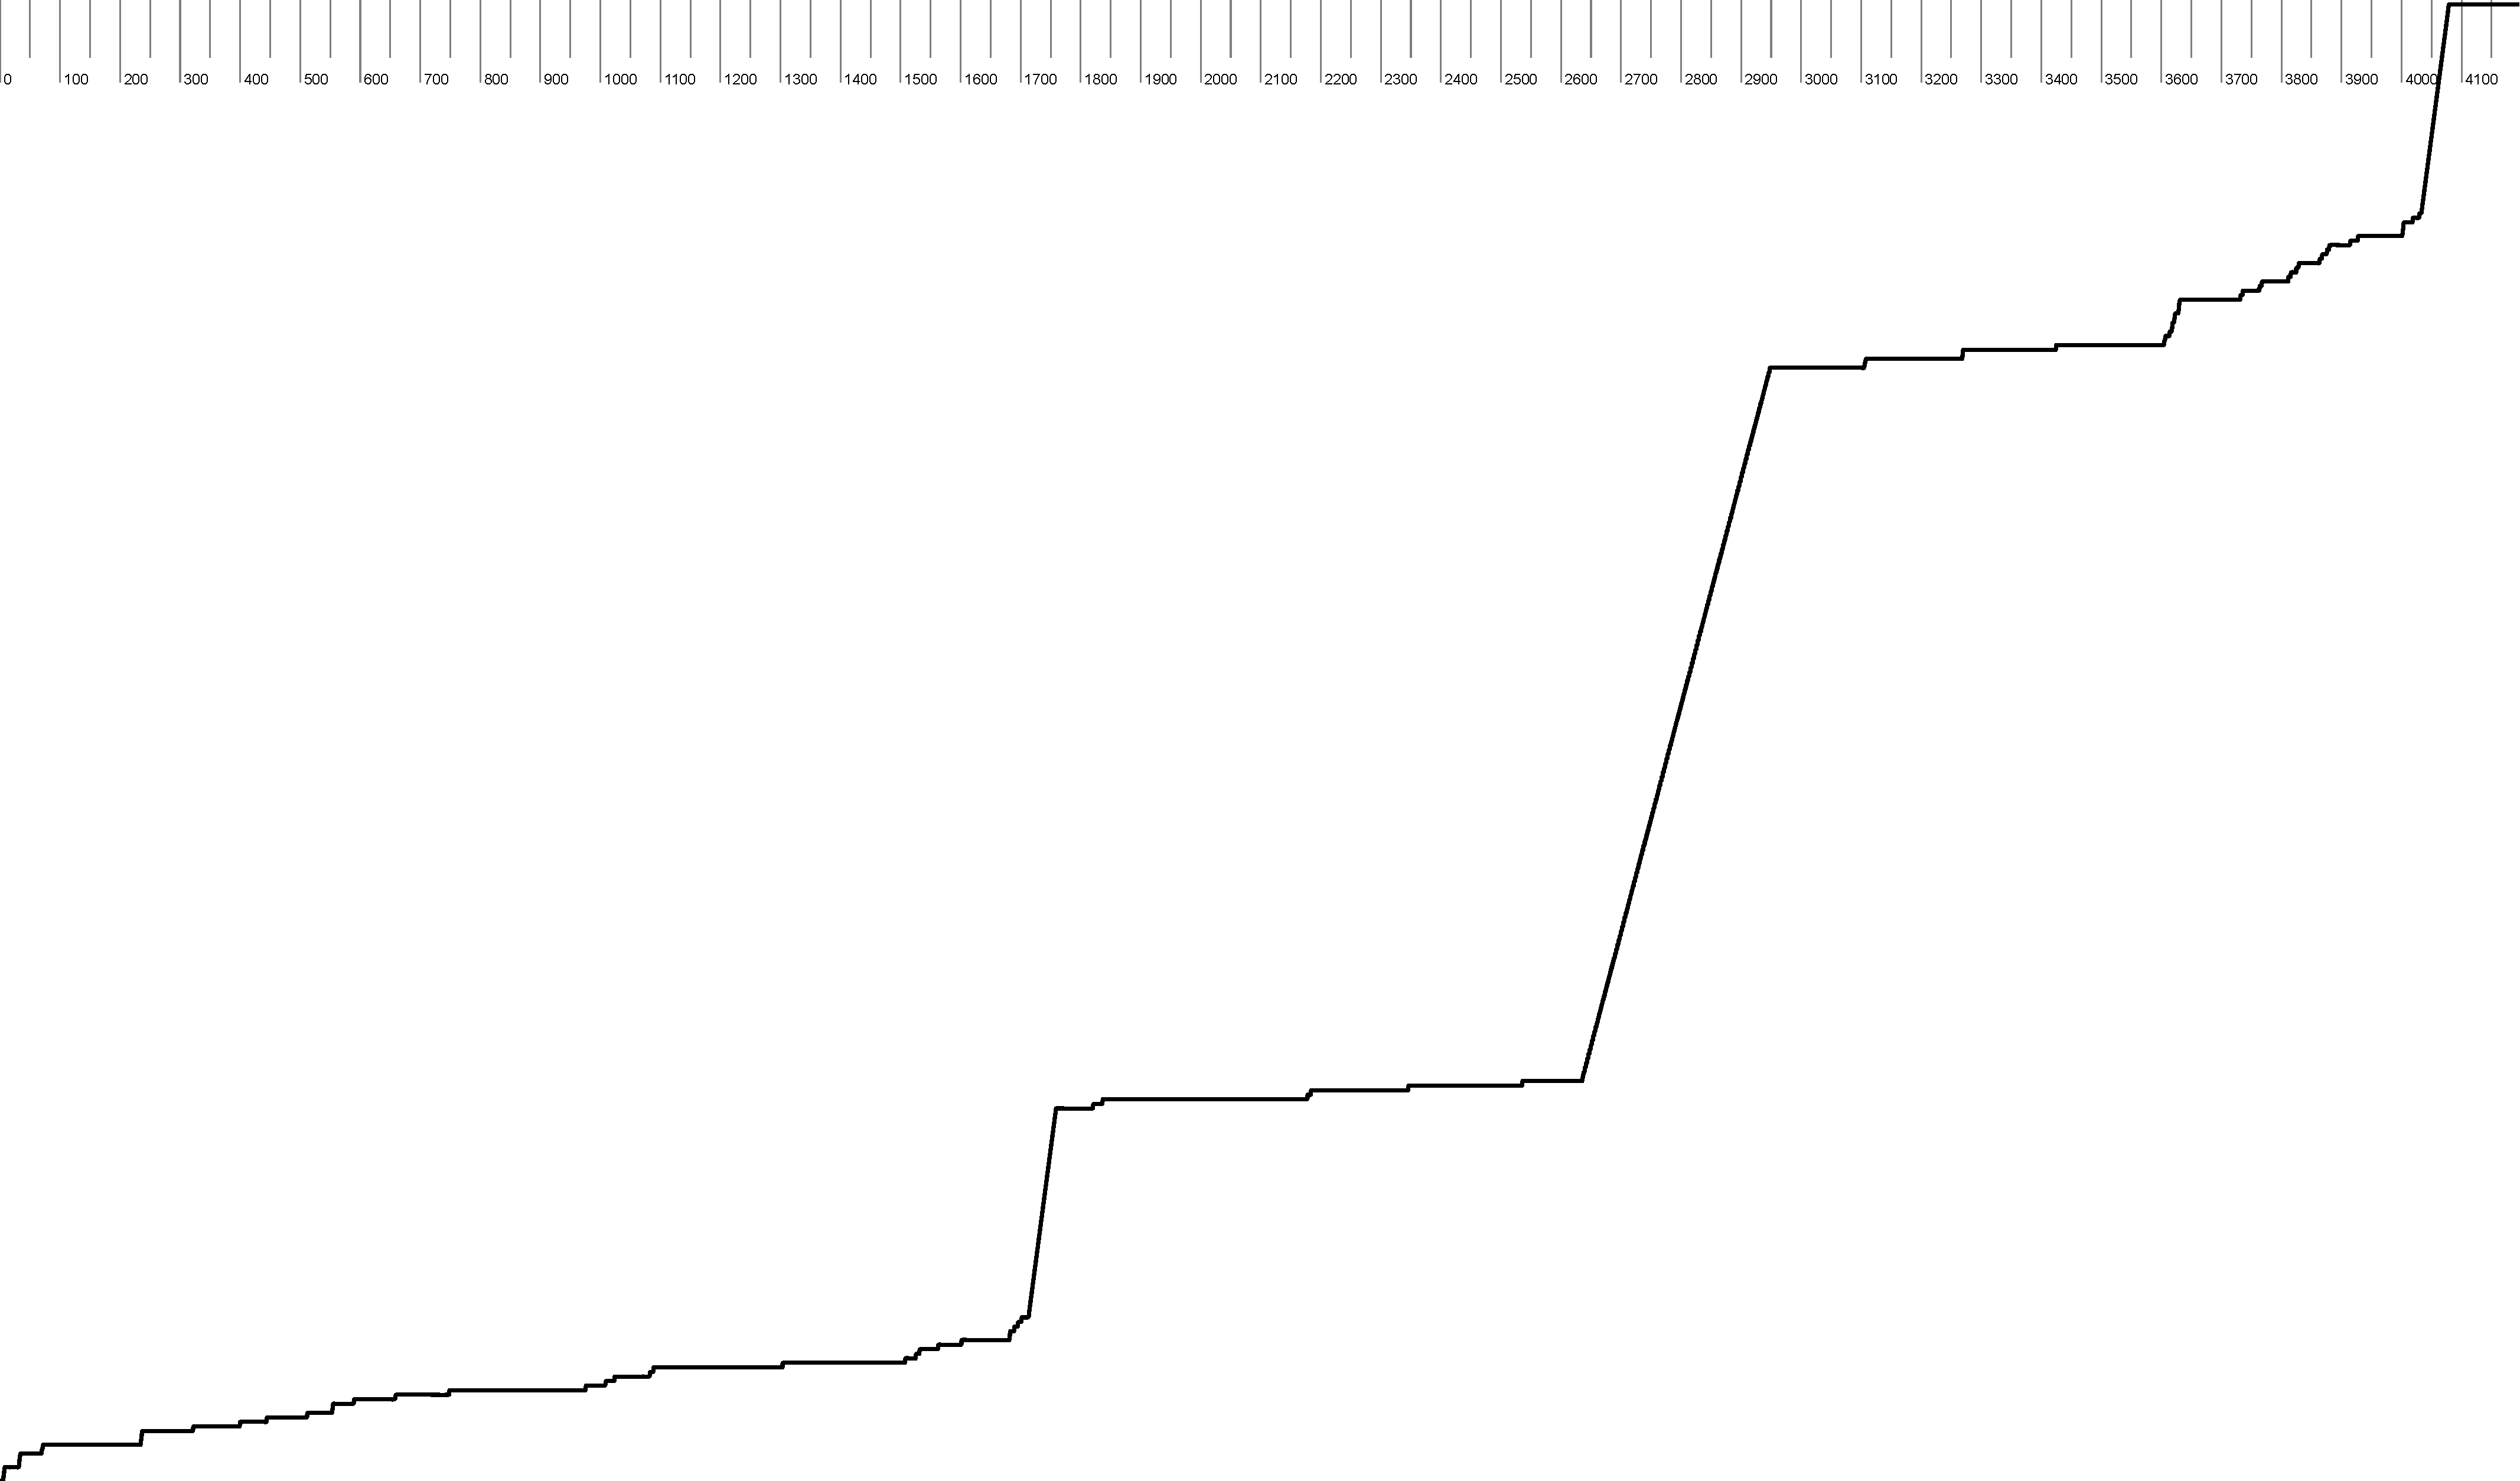
\includegraphics[width=0.95 \linewidth]{mario-global}
\end{center}\vspace{-0.1in}
\caption[lof not used]{
  A single maximal tight valid lexicographic ordering for my
  4,000-frame input training data to Super Mario Bros.. This function
  is globally nondecreasing, and is the decimal memory locations
  $\langle$\!~232, 57, 73, 74, 75, 115, 130, 155, 32, 184, 280,
  491, 506, 1280, 1281, 1282, 1283, 1288, 1290, 1337, 1338, 1339,
  1384, 1488, 1490, 1496, 1497, 1498, 1499, 1514, 1873, 1882, 1888,
  1904, 1872, 1906, 112, 113, 114, 2009, 2010, 2011, 1539~\!$\rangle$.

  This is not a great objective function; there are long spans where
  all the memories are equal according to it, and the nice smooth slopes
  are happening during level transitions where the game is ignoring
  inputs (they are probably timers counting up each frame, which is
  why they are so smooth). Other slicing produces better objectives.  

  For reasons unknown---I just discovered this while generating the
  figure---{\em all} of the objective functions learned with this
  method, regardless of the nondeterministic choices, appear to have
  this same curve, despite using different memory locations. It may be
  that they are different permutations of bytes that all change
  simultaneously, only on the frames where there are jumps in this
  picture, and there are no other orderings that are tight, valid, and
  maximal. This is still surprising and warrants investigation. }
\label{fig:global}
\end{figure}

\begin{figure}[htb]
\begin{center}
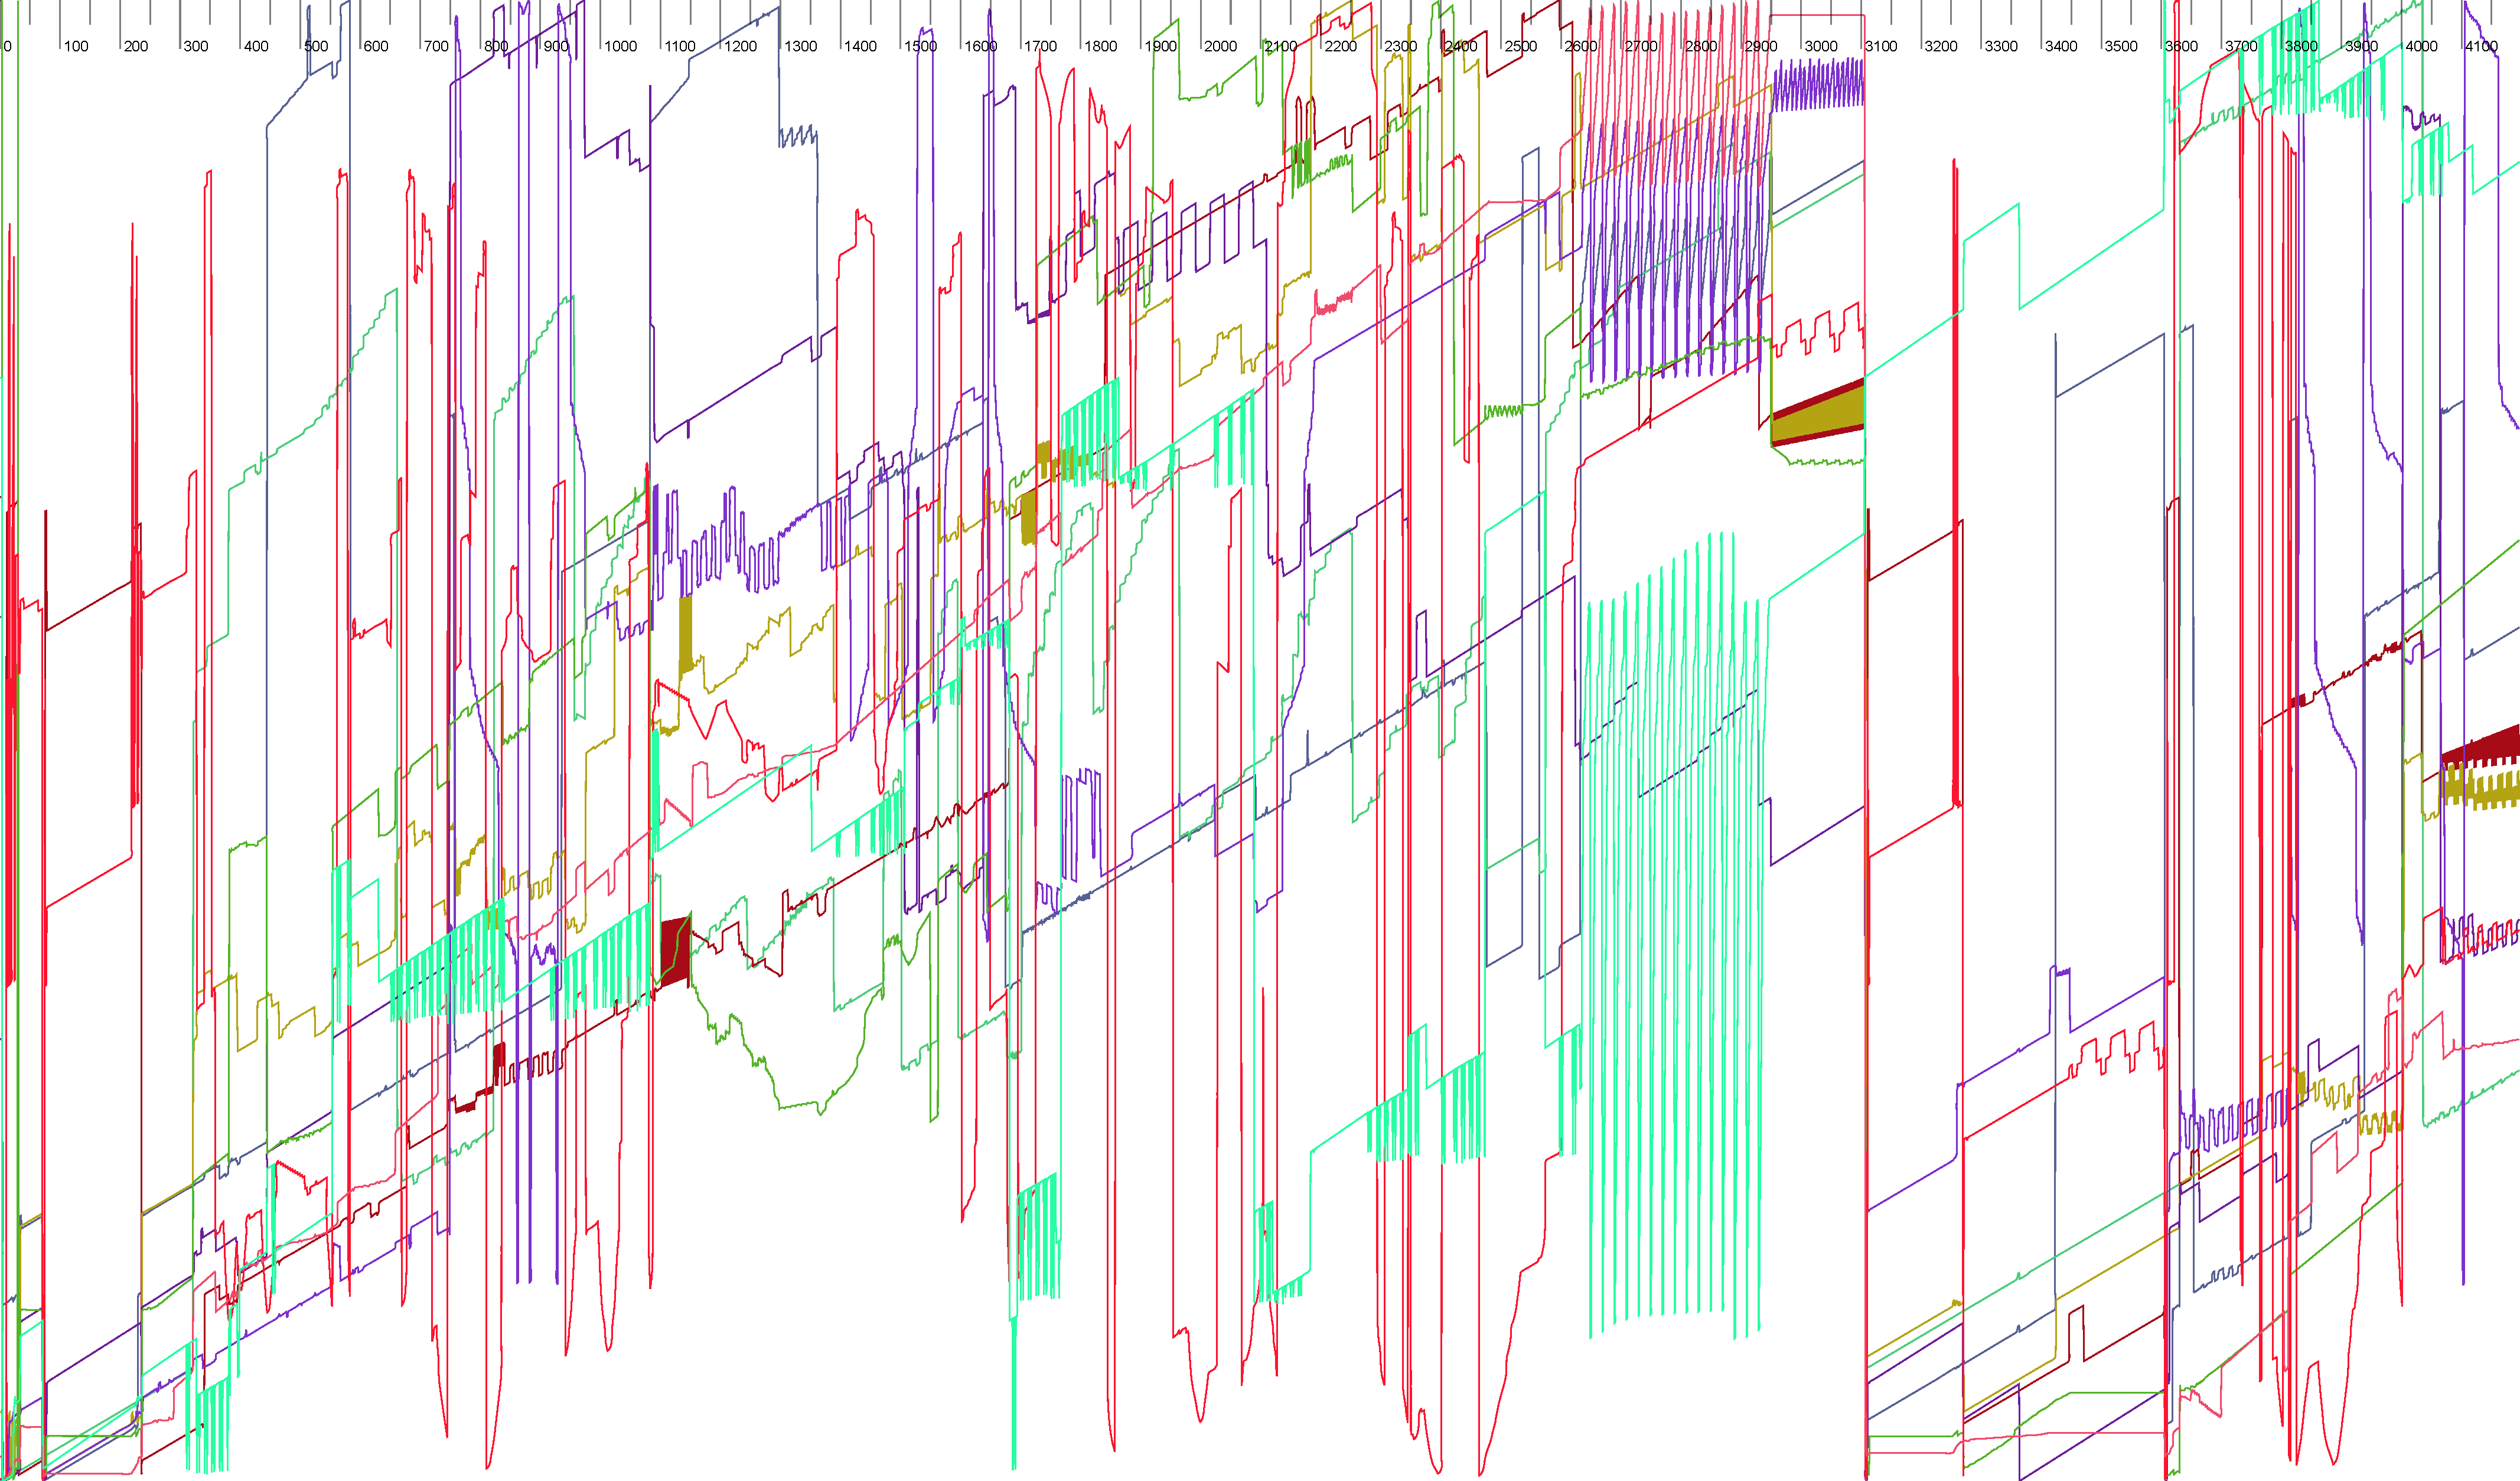
\includegraphics[width=0.95 \linewidth]{mario-tenths}
\end{center}\vspace{-0.1in}
\caption{Ten objective functions trained on different tenths of the
  4,000 inputs for Super Mario Bros.. These functions are normalized
  against the range of all values they take on during the movie; you
  can see that most are increasing locally most of the time, but many
  drop back to zero around the 3100\th\ frame, when Mario reaches
  world {\tt 1-2}. Within its 400-frame window, each objective is
  guaranteed to be nondecreasing.}
\label{fig:tenths}
\end{figure}

\begin{figure}[htb]
\begin{center}
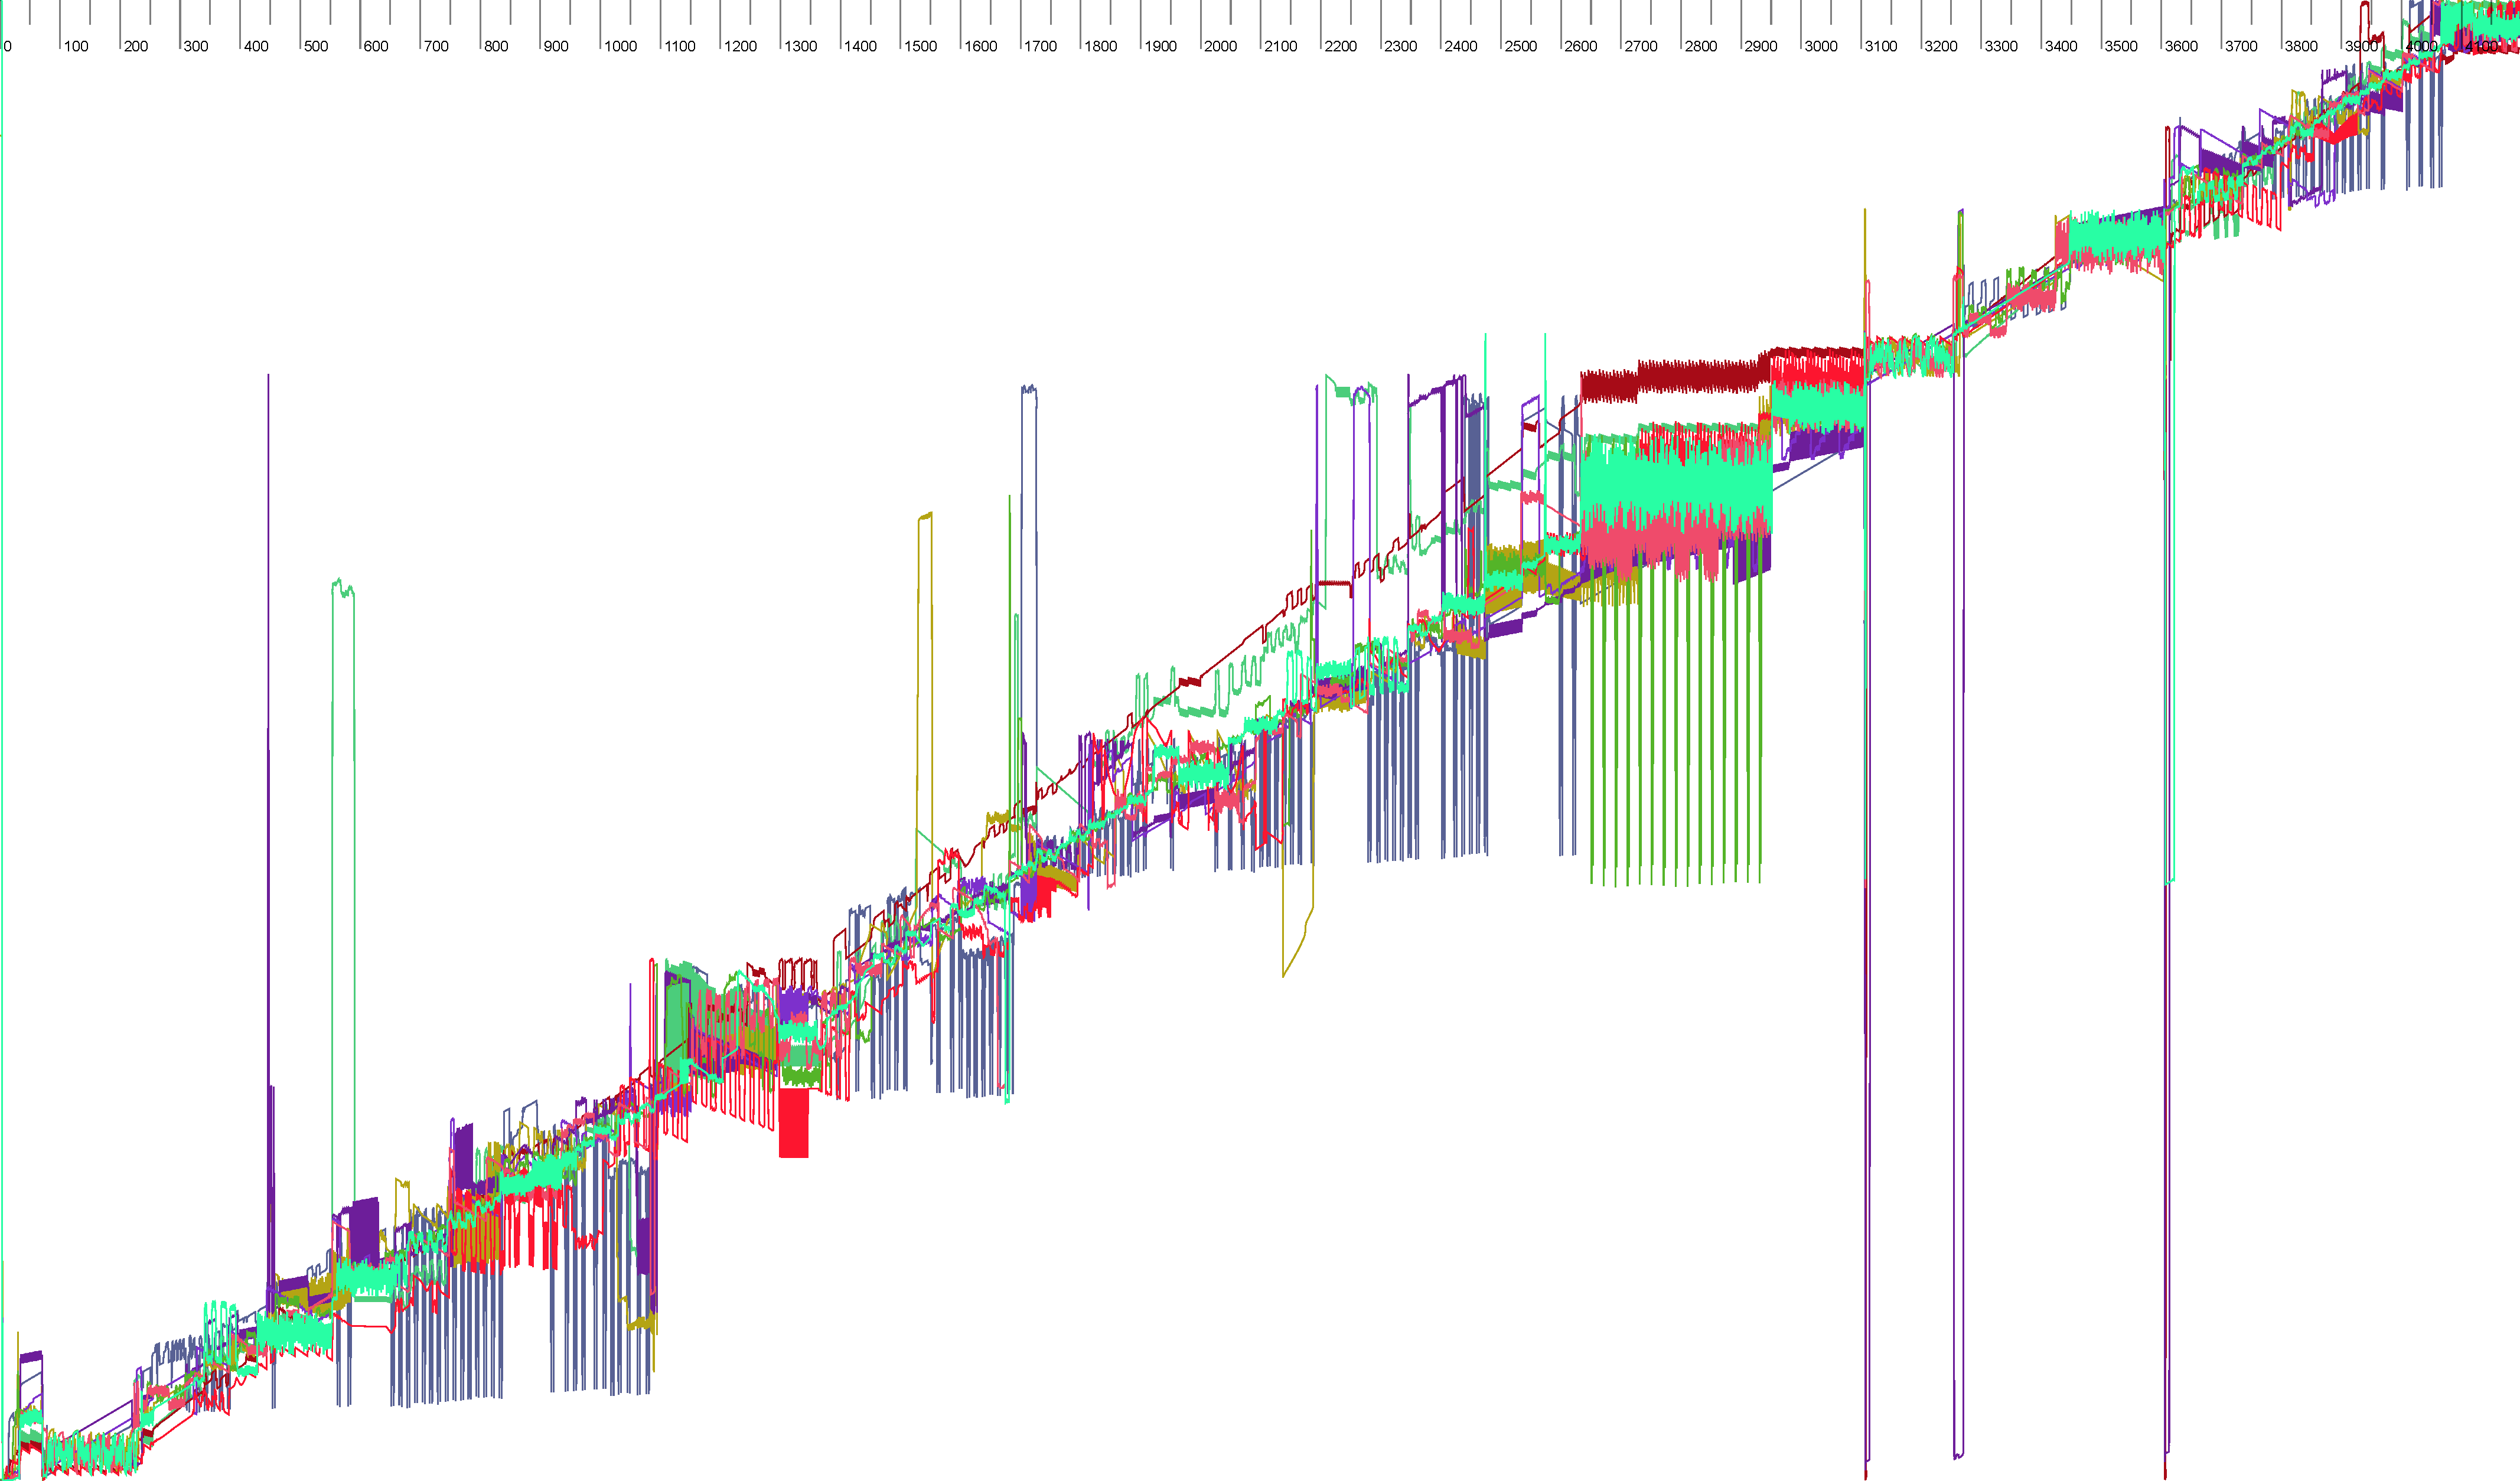
\includegraphics[width=0.95 \linewidth]{mario-strides}
\end{center}\vspace{-0.1in}
\caption{Ten objective functions trained on every 100\th\ memory,
  starting at frame 0, frame 1, and so on up to frame 10. Normalized
  as usual. These objectives exhibit excellent global progress, but
  are locally very noisy. Among the methods I used to generate
  objectives, this one produces the best results (based on my
  intuition about what a good objective function looks like).
}
\label{fig:strides}
\end{figure}

In order to derive an objective function, we'll start with an abstract
subroutine that finds a single lexicographic ordering
nondeterministically. This function takes in an ordered list of $n$
memories $M_1\ldots M_n$ which all have size $m$ bytes. For example,
$m = 2048$ and $n = 100$, for the memories at each of the first $100$
frames of someone playing Super Mario Bros.. It produces an ordered
list of unique memory locations $L_1 \ldots L_k$ (where $0 \leq L_i <
m$, that is, each is some spot in the 2048 bytes of RAM) that is a
{\em maximal} {\em tight} {\em valid} lexicographic ordering of $M$.
Let's start by defining those terms just to be careful.

Given some list of memory locations $L_1 \ldots L_k$ and a pair of
memories $M_a$ and $M_b$, we say that $M_a =_L M_b$ iff $M_a[L_1] =
M_b[L_1]$ and $M_a[L_2] = M_b[L_2]$ and so on for every $L_i$; that
is, the bytes must be equal at each of the locations. Easy. We say
that $M_a <_L M_b$ iff there exists some $p \leq k$ where $M_a[L_1] =
M_b[L_1] \ldots M_a[L_{p-1}] = M_b[L_{p-1}]$ and $M_a[L_p] <
M_b[L_p]$. Put simply, if the two memories are not equal according to
$L$ (have the same byte at every memory location) then there is a
unique first location ($L_p$) where they have a different byte, and
that byte determines the order. $M_a >_L M_b$ is just defined as $M_b <_L
M_a$; $M_a \leq_L M_b$ is just $M_a <_L M_b$ or $M_a =_L M_b$, and similarly
for $\geq_L$, and they mean what you think so don't worry.

Every $L$ defines a lexicographic ordering ($<$ and $=$ operators).
$L$ is a {\em valid} lexicographic ordering of $M$ if $M_i \leq_L M_{i
  + 1}$ for $1 \leq i \leq n$; each memory is less than or equal to
the next memory in the sequence. It follows that $M_i \leq_L M_j$
whenever $i < j$.

Every prefix of a valid $L$ (including the empty prefix) is a valid
lexicographic ordering as well. On a scale from useless to useful, the
empty prefix is a 1 (it equates all memories), which suggests that
some orderings are better than other. To give a primitive notion of
``good'' lexicographic orderings, we define a {\em maximal} valid
lexicographic ordering to be $L$ such that there are no extensions of
$L$ that are valid. An extension of $L_1 \ldots L_k$ is just $L_1
\ldots L_k, L_{k+1}$ (where $L_{k+1} \neq L_i$ for $1 \leq i \leq k$):
Some new memory location that we put at the end of the order (in the
least important position). We do not consider extending in the middle
of the order or beginning, although that would make sense.

Maximal valid orderings are good and it is straightforward to produce
them (a less constrained version of the algorithm below), but they
have the bummer downside that memory locations that never change value
for any $M$ can be included at any position of the ordering, and all
such choices are equivalent. And in fact all locations {\em must} be
included to make the ordering {\em maximal}. This is bad because when
$M$ contains many locations with fixed values, we have boatloads of
equivalent orderings, and they're also longer than necessary. An {\em
  tight} valid ordering is one where for each $L_i$ there exists at
least one $M_a$ and $M_{a+1}$ where $M_a[L_i] < M_{a+1}[L_i]$ and
$M_a[L_j] = M_{a+1}[L_j]$ for all $i < j$; that is, every location has
to participate in the ordering at least once. The notion of {\em
  maximal} has to be relative to this property as well---a {\em tight
  extension} is one that produces a tight valid ordering, and a {\em
  maximal tight valid ordering} permits no tight extensions.

On a scale from simple to fancy, the algorithm to generate $L$ from
$M$ is a 3. Given those definitions, the idea is to start with the
empty prefix, which is always a tight valid lexicographic ordering but
usually not maximal. We then pick a tight extension that is valid; if
none exists then we are done and have a maximal tight valid ordering.
Otherwise we have a new tight valid ordering, and we repeat.

The pseudocode gives a pseudoimplementation of the algorithm that is
more pseudodetailed. The C++ implementation is in \verb+objective.*+.
C++ is not a good language for this kind of program but we use it
because the NES emulator is written in C++.

\begin{figure*}[htp]
  \begin{code}
    (* Prefix is the prefix so far (int list) and remain is the list of memory
       locations that we can still consider. Invariant is that prefix is a
       tight valid ordering on $M$. Returns the memory locations from remain 
       that are a tight extension of the prefix. *)
    fun candidates (prefix, remain) =
      let lequal = (* list of indices $i$ where
                      $M_i =_{\tt\! prefix} M_{i+1}$ *)
      let notgreater = (* members $x$ of remain where
                          $M_i[x] > M_{i+1}[x]$ is
                          not true for any $i$ in
                         {\tt lequal} *)
      let tight = (* members $y$ of notgreater where
                     $M_i[x] < M_{i+1}[x]$ is true
                     for some $i$ in{\tt lequal} *)
      in tight

    \

    (* Returns a maximal tight valid ordering, given a tight valid prefix and 
       list of memory locations we are permitted to consider. *)
    fun ordering (prefix, remain) =
      case candidates (prefix, remain) of
        (* No extensions means it's maximal. *)
        nil => prefix
      | cand =>
        let c = nondeterministically-choose-one cand
        let remain' = remove-element (remain, c)
        let prefix' = prefix @ [c]
        in ordering (prefix', remain')
  \end{code}

  \caption{Pseudocodes for nondeterministically generating a maximal
    tight valid lexicographic ordering on some memories $M$. The
    recursive function {\tt ordering} just orchestrates the selection
    of an extension until there are no possibilities remaining, and
    returns it. The function {\tt candidates} finds all the possible
    extensions for a prefix. First we compute {\tt lequal}, all of the
    adjacent memory pairs (represented by the index of the first in
    the pair) where the memories are equal on the prefix. Only pairs
    that are equal on the prefix are interesting because these are the
    only ones that will even depend on the extension to the prefix
    when comparing the memories. We only need to consider adjacent
    pairs because on an a scale of exercise for the reader to proof is
    contained in the extended technical report, this statement is a
    you can figure that one out yourself. Valid extension locations
    are ones where the memory pairs are never increasing at that
    location (note that in places where pairs are not equal but
    strictly less on the prefix, it's perfectly fine for the extension
    to be greater; this is the ``point'' of lexicographic orderings).
    Finally, tight extensions are those valid ones that have at least
    one pair of memories where the location has a value that is
    strictly less.}
  \label{fig:ordering}
\end{figure*}

\subsection{The objective function, in practice}

We can't just use a single objective function. Choosing objective
functions nondeterministically, we may get a crap one like ``High byte
of the score'' which only goes up once during all of our memory
observations. We also can't just use all of the memory observations,
because there may be brief moments that violate strict orderings, like
Mario's $x$ coordinate temporarily decreasing to navigate around an
obstacle. More starkly, the first few hundred frames of the game are
almost always initialization where the memory temporarily takes on
values that are not representative of later gameplay at all. In
practice, we use the nondeterministic function from
Section~\ref{sec:deriving} on multiple different slices of the memory
observations. We also call it many times to nondeterministically
generate many different objectives. Finally, we weight the objectives
by how representative we think they are.

\parameteralert{This one of the first places where we have some
  arbitrary constants, which are the enemy of elegance. On a scale of
  ballpark to obsessively overfit, these constants are a 2; I
  basically looked at some graphs while developing the objective
  function learning part of the code to decide whether they were
  ``good enough'' and didn't tune them after starting to observe
  actual performance. Some of those graphs appear in figures here.
  For all I know, these are really bad choices, but it was important
  for aesthetic reasons for the objective function to be brutish. The
  only reason to permit these parameters at all is that it simply
  does not work to have a single ordering or to use only orderings
  that apply to the whole memory.}

\paragraph{Skipping.} To avoid being confused by RAM initialization and
menu, I ignore all memories up until the first input by the player.
Including these would be especially suspicious because the RAM's
contents are not even well-defined until the program writes something
to them.\footnote{Emulators tend to fix them to a specific pattern so
  that emulation is completely deterministic, but in real hardware
  they are truly uninitialized, or retain the values from the last
  reset or game inserted. Some semi-famous tricks involve removing and
  inserting game cartridges while the system is running in order to
  take advantage of this.}

\paragraph{Slicing.} I generate 50 orderings for $M_1 \ldots M_n$; the
whole recording starting immediately after the first keypress. During
gameplay some values really are completely nondecreasing, like the
player's score and world/level pair. Figure~\ref{fig:global} shows
what a global ordering looks like. I also generate 3 orderings for
each tenth of the memory sequence, e.g. $M_1 \ldots M_{n/10}$ and
$M_{n/10+1} \ldots M_{2n/10}$, etc. The intention is to capture
orderings that are rarely violated, or sections of the game with
unusual objectives (e.g. a minigame or swimming level). Orderings
generated this way look pretty random, and on a scale from solid to
suspicious, I can't vouch for them. Then I generate objectives from
non-consecutive memories that are evenly spread out through the
observations: Ten objectives chosen from every 100\th\ memory,
starting from the 0\th\ frame, 1\st\ frame, 2\nd\ frame, and so on up
to the 9\th{}. Similarly for every 250\th\ frame, and a single
objective for memory sliced to every 1000\th\ frame, with start
positions of 0--9. The intention is to capture objectives that grow
slowly over the course of a playthrough, without getting distracted by
local noise.

\paragraph{Weighting.} \label{sec:objectiveweighting} 
To reduce the importance of randomness in the
learning process, and the arbitrariness of the slicing, each objective
function is also assigned a weight. An ideal objective function takes
on its minimal value on the first frame and maximal on the last
(according to the ordering), and increases steadily throughout the
observed memories. This is ideal because it allows us to just follow
the gradient to reach good states. A bad objective function freqently
regresses (recall that although we produce valid orderings, an
ordering that is valid on some slice may not be valid for the whole
sequence of memories). To weight an objective $L$, we first collect
all of the values (the vector of values of the memory locations $L_1
\ldots L_k$) it takes on throughout the observations. These may not
obey the ordering. We then sort the values lexicographically and
remove duplicates.\footnote{Note to self: I'm not sure how to justify
  removing duplicates here. It makes [0, 1, 1, 1, 1, 1, 10, 11] look
  the same as [0, 1, 10, 11], which is probably not desirable?} Call
this $V$. Now we can compute the {\em value fraction} for $L$ on some
$M$: Extract the vector of locations $M[L_1], M[L_2], \ldots, M[L_k]$
and find the lowest index $i$ in $V$ where the vector is less than or
equal to $V_i$. The value fraction {\tt VF} is $i/|V|$, which is the
normalized value of ``how big'' $M$ is, according to $L$, compared to
all the values we ever saw for it. The value fraction is defined and
in $[0, 1)$ for all memories in the observed set.\footnote{It is not
    defined when the memory is greater than all observed memories,
    which we will encounter later. The code returns $|V|/|V| = 1$ in
    that case, which is as good as anything.} This gives us the
  ability to compare objectives on an absolute scale.\footnote{This is
    certainly not the only way to do it, and it has some questionable
    properties like ignoring the magnitude of change. But it is very
    simple.} Weighting an objective is now simple:
%
$$ \Sigma_{i=1}^{n-1}  {\tt VF}(M_{i+1}) - {\tt VF}(M_{i}) $$
%
We sum the differences in value functions for each consecutive pair of
memories. In the case of the ideal function this is $\Sigma_{i=1}^{n-1}
1/n$, which approaches $1$. Of course, when you think about it,
this is actually the same as
%
\[
\begin{array}{c}
({\tt VF}(M_1) - {\tt VF}(M_0)) + ({\tt VF}(M_2) - {\tt VF}(M_1)) \,+ \\
\vdots \\
({\tt VF}(M_{m-1}) - {\tt VF}(M_{m-2})) + ({\tt VF}(M_{m}) - {\tt VF}(M_{m}))
\end{array}
\]
%
and all but $-{\tt VF}(M_0)$ and ${\tt VF}(M_m)$ cancel out. This
means that the weight we use is just the final value minus the initial
value, regardless of what happens in-between.\footnote{I think this
  can be improved, for example by taking the deviation from the ideal
  linear objective.} The mean value theorem or something is probably
relevant here. {\bf Lesson about being careful:} I only realized that
this code was kind of fishy when I started writing it up for SIGBOVIK.
Not only did it loop over all the deltas as in the $\Sigma$ expression
above, but it also summed from $i=0$ and kept track of the last value
fraction at each step, thus treating the value fraction of the
nonexistent memory $M_0$ as 0. This is wrong, because the first value
fraction may be very high, which credits the objective with a positive
value (e.g. 1) for that first part of the sum. Objectives that start
high on the first frame are not ideal; in fact, the worst objectives
start high on the first frame and steadily {\em decrease}. After
writing this up I corrected it to the simple expression ${\tt VF}(M_m)
- {\tt VF}(M_0)$ and the result was a huge breakthrough in the
quality of the output! I had spent much time tuning the {\tt
  playfun} search procedure (Section~\ref{sec:playfun}) and not
investigated whether the objectives were being weighted properly. More
on this later, but the lesson is: Bugs matter, and thinking about your
code and explaining it is a good way to find bugs.

Objectives are constrained to have non-negative weights (I set the
value to 0 if negative, which effectively disables it). We save the
objectives and their weights to a file and then we are done with the
easy part.

\subsection{Motifs} \label{sec:motifs}

The very first thing I tried with the objective function is to just do
some greedy search for input sequences that increased the objective.
This works terribly, because the search space for inputs is large
($2^8$ possibilities at each frame). Most are useless (it's almost
impossible to press the left and right directions at the same time,
and real players almost never do it); real input sequences usually do
not change values 60 times per second (rather, the player holds the
jump button for 10--20 frames); some button-presses and combinations
are much more common than others (e.g. right+B is common for running
right, but start pauses the game). Search quickly necessitates a model
for inputs. Rather than do anything custom, I just use a really dumb
approach: Take the observed inputs (the same ones that we learned the
objective functions from) and split them into chunks of 10 inputs.
Motifs are weighted by the number of times they occur in the input.
There may be a single motif at the end that's fewer than 10 inputs.

\parameteralert{Here I choose the magic number 10 for the size of input
  motifs. On a scale from gravitational constant to pulled it out of
  my ass, this is an 8. We could perhaps justify 10 as being close to
  the speed of input change actually possible for a human (6 button
  presses per second; 166ms). I believe it is possible to do much
  better here and the code contains a few such false starts, but using
  motifs was one of the biggest immediate improvements in the history
  of this code, so I went with it. A natural thing to try is a Markov
  model, although this has a free parameter too (the number of states
  of history). It is likely possible to do some kind of abstract
  interpretation where multiple different input sequences with
  equivalent outcomes are explored simultaneously, which might obviate
  the need for computing an input model from the observed play. The
  playfun algorithm below takes motifs as primitive because of the way
  it was developed; I'll use footnotes to describe my thinking about
  how to remove this.}

Motifs are written to a file too and then we're done with that. This
concludes the learning we do from the example input; everything else
is a matter of using the objective functions and motifs to play the
game.

\section{Now you're playing with power} \label{sec:playfun}

In this section I'll describe how the objective functions are used to
play the game. On a scale from canonical to Star Wars Christmas
Special, this algorithm is an 7. So, rather than focus on the
particulars of some of the heuristics, I'll try to give a story of the
different things I tried, what motivated the ideas in the current
version, and my intuitions about what is working well (or not) and
why. This algorithm is called {\tt playfun} and it can be found
implemented in C++ in {\tt playfun.cc}; some historic versions are
in {\tt playfun-*.cc}.

\subsection{Basic software architecture}

In order to use the emulator to search for good sequences of inputs, I
needed deeper integration than just observing memory. The FCEUX
emulator is about a jillion lines of C++-ish code, was intended as an
interactive GUI application, contains support for multiple different
platforms, and the code is, on a scale from a pile of horse shit to
not horse shit, approximately a 2.\footnote{It is, however, an
  excellent emulator to use, has fancy tools for recording and editing
  movies, and is popular in the speedrun community. I highly recommend
  it; just don't read the code.} With a medium amount of suffering I
got the emulator compiling under mingw in 64-bit mode, and working
behind a streamlined interface ({\tt emulator.h}). Once a game is
initialized, it is always at an input frame---you can give it an 8-bit
input (for the 1\st\ player) to step a single frame, or read the 2048
bytes of memory. You can also save the complete state of the emulator
into a vector of bytes, which allows you to restore the state to
exactly that same point.\footnote{This contains the RAM, but also
  stuff we didn't consider, like registers, the Picture Processing
  Unit's state, and internal emulator stuff.} These save-states are
portable across sessions as long as the code was compiled and the game
initialized the right way.\footnote{The original FCEUX supports
  portable save-states, but I removed that guarantee in order to get
  the smallest possible byte vectors. More on that below.} FCEUX must
be single-threaded because it uses global variables galore. I made
several enhancements to the emulator interface, which are discussed
later.

It's important to know that almost all the CPU time in all the
algorithms discussed in this paper is spent emulating NES frames; it
takes about 500\textmu s to process a single step. Lots of engineering
effort goes into reducing the number of frames the algorithms emulate.
The {\tt playfun} program takes a ROM file, the learned objectives and
motifs, and runs on the console for arbitrarily long, outputting a
movie file consisting of the input sequence it think is best. The
current {\tt playfun} algorithm is much too slow to run real-time, but
it would be possible to have video output as it played. I disabled
most of the video code, however, in an effort to make the emulation
loop run as fast as possible.

\subsection{Naive attempts} \label{sec:naive}

The very first thing I tried, as mentioned in
Section~\ref{sec:motifs}, was to just look at all $2^8$ different
possible inputs at each step, and pick the best one. The inner loop
looks pseudolike this:

\begin{code}
for (;;) \{
  vector<uint8> before = GetMemory();
  vector<uint8> state = GetState();
  // Try every bitmask of the 8 inputs.
  for (int i = 0; i < 256; i++) \{
    RestoreState(state);
    Step((uint8)i);
    vector<uint8> after = GetMemory();
    double score = Score(before, after);
    // Save the best-scoring i...
  \}
  RestoreState(state);
  Step(bestinput);
\}
\end{code}

{\tt Score} computes a score of two memories using the objective
functions, which was the point of all that. There are a few
canonical-seeming ways to implement this; the simplest is to
count the (weighted) number of objective functions $o$ where
${\tt before} <_o {\tt after}$. We'll get to more later.

I wish this worked, because that would be truly laughable (and is fast
enough to run real-time), but on a scale from doesn't to does it's a
1. At best, Mario twitches in place. The inputs that it plays are
insane. There are lots of reasons, but a clear one is that a single
input rarely affects your progress in the game on the very next frame.
I didn't really expect this approach to work and I already knew that
the state space is too big to search exhaustively, which is why I
implemented motifs. This drastically reduces the search space and
makes each step more significant; the inner loop can now be:

\begin{code}
for (const Motif &m : motifs) \{
  RestoreState(state);
  for (uint8 i : m.inputs()) Step(i);
  vector<uint8> after = GetMemory();
  double score = Score(before, after);
  // Save the best-scoring motif...
\}
\end{code}

This works much better (anything would), though not much better than
you'd expect from just weighted random playback of the motifs
themselves (they mostly contain motifs like ``hold right'' and ``hold
right and A''). Mario is bad at avoiding danger except by luck, and
bad at jumping hard enough to get over pipes (the button needs to be
held consecutively for maybe 40--50 frames to jump that high).

These two things---danger avoidance and microplanning to string
together multiple motifs in a useful way---are two sides of the same
coin. At least, on a scale from one side of the coin to the other, it
is a two. My attempts to address these two problems converged on a
single idea that is the crux of the good part of {\tt playfun}. First
let's start with avoiding bad futures, since that is somewhat simpler.

\subsection{Avoiding bad futures}

Scoring a move based on how much better it is than the previous state
causes Mario to make sensible greedy moves to increase the objective
function---until he is then faced with no good options. This happens
very frequently in Super Mario Bros.~(and many other games) because
death is not usually a single-frame affair. For example, once he's
near a Goomba with some velocity, it's too late to slow down or jump
out of the way; he'll die in a few frames. Similarly, he can be in the
midst of a too-short jump over a pit, where he's destined to die no
matter how he squirms. Moreover, in Mario and many other games, even
death as recognizable to the player isn't an obvious loss to these
objective functions; the game's memory doesn't change much until the
interstitial screen and Mario being reset back to the nearest
checkpoint. So in order to avoid danger, Mario needs to avoid states
that make death a foregone conclusion, not just avoid death.

This is nothing special; move search in Chess and pretty much any game
involves evaluating an ending game state and not just the quality of
the move itself (``I captured a piece! Must be a great move!'').
Evaluating a Chess state is a delicate matter, but Goombas and gravity
are very stupid opponents. For avoiding danger, the following works
well: Take the state and run a few seconds (300--500 frames) worth of
weighted random motifs, several times. This gives us a set of states
that could follow our candidate state were we to keep playing. We
judge the candidate state not on its immediate value compared to our
start state, but based on the random futures that may ensue. In my
first version I used the minimum value of all these random futures, so
that if Mario was getting into a state where he could die, those
states would have low scores. Later we'll find that this isn't the
right way to think about it, but it gives us a big improvement in the
quality of play---Mario cleanly jumps over Goombas. He also gets very
nervous and all like analysis-paralysis when faced with pits of medium
size\footnote{The companion website contains videos of this, which are
  funny. \url{http://tom7.org/mario/}}, which is related to the next
section.

\subsection{Seeking good futures}

The flipside of avoiding danger is seeking adventure. Mario can avoid
danger for quite a long time by just waiting at the beginning of the
game, until time runs out. He can dilly dally before a pit,
contemplating the void. But princesses need rescuin'. The same
approach as before works for evaluating a state in terms of its
potential: Try some random futures and look at where we end up. We
could take the max over those scores if we're being optimistic, or the
average or sum if we're trying to judge the general value of the
state. In my first version, which did work pretty well, I took the
max; so basically I had the min of some random states plus the max of
some other states. But why generate a bunch of futures and take the
min of some and the max of some others? On a scale of Thank You Mario
Your Quest Is Over We Present You A New Quest Push Button B to I'm
Sorry, but Our Princess is in Another Similarly-Shaped but Not Exactly
that Samesuch Castle, this is an 8.

\subsection{Stable futures}

Taking the minimum of random futures is always silly (at least if we
believe our objective function), because nothing other than our own
bad memory can force us to take a series of steps if we know a
different better series of steps. Taking the max is possibly foolish
if we don't know how to reconstruct a rare good state that caused the
maximum score to be high. Both lead us to the idea: Keep around a set
of candidate futures that we use for evaluation and search, rather
than just randomly generating futures when we want to evaluate a state
and then discarding them. This turns out to work really well and be
more efficient.

The basic version of the {\tt playfun} algorithm looks like this.
Maintain {\tt NFUTURES} futures (this is 40 for the results presented
in Section~\ref{sec:results}), originally just seeded with weighted
random motifs. We aren't likely to execute any of these futures
verbatim, but they are intended to give us high watermarks of what
we're capable of, plus allow us to judge future danger. As we execute
search, futures will be partly consumed and extended, and some discarded
and replaced.

Each future stores a desired length from 50--800 frames, and whenever
it is shorter than that, we extend it (at its end) with random weighted
motifs. The inner pseudoloop then looks like this:

\begin{code}
for (;;) \{
  vector<uint8> before = GetMemory();
  vector<uint8> state = GetState();

 \ 

  set<vector<uint8>> nexts;
  for (Future f : futures) \{
    nexts.insert(f.First10Frames());
    f.ChopOffFirst10Frames();
  \}

 \ 

  while (nexts.size() < NFUTURES)
    nexts.push\_back(/* random motif */);

 \ 

  for (vector<uint8> &next : nexts) \{
    RestoreState(state);
    for (uint8 i : next) Step(i);
    double score =
      ScoreByFutures(before, futures);
    // Save the best-scoring next...
  \}

 \ 

  ReweightMotifs(best\_next, motifs);
  ReplaceBadFutures(futures);
  ExtendFuturesToDesiredLengths(futures);
\}
\end{code}

At each iteration of the loop we will find the best next 10-frame
sequence to commit to. Rather than search over all motifs, we search
over the first 10 frames of each future. This has several important
consequences. First, since futures are generated by weighted motifs,
it makes it more likely that we spend CPU time evaluating motifs that
are common; the code from Section~\ref{sec:naive} always explores
every motif, even rare ones. Second, it guarantees that if we pick
some 10 frames on the basis of a single good future, we don't have to
worry about recreating that future; it will still be among our futures
for the next round. This is key: It allows us to use the determinism
of the game to replay a really good future if we find one, not just
use average random futures to assess how good a state will be.

The function {\tt ScoreByFutures} saves the state, then runs each
of the {\tt NFUTURES} futures to get a final state and memory. We
score each final memory relative to the start memory. The particulars
of scoring are not as interesting as the general idea, which is:
\begin{itemize}
\item The potential 10-frame {\tt next} sequence that we're
evaluating gets an {\em optimistic} score. This is based on the futures
for which the objectives {\em go up}. This is always non-negative.
\item Each future is also given a score, which is the sum of scores
from all the different {\tt next} sequences, regardless of their sign.
\end{itemize}

The purpose of the first is to identify a good {\tt next} sequence. We
take the sequence with the highest optimistic score. The idea is that
this is the sequence that gives us the best outcome if we continue
to control what we do in the future.

The purpose of the second is to identify which futures are good. A
good future tends to bring good outcomes regardless of the immediate
next step. Random futures that make is walk left when the good stuff
is to the right, or jump when there are spikes nearby above our head,
will receive negative scores for many or all of the {\tt next}
sequences.

{\tt ReweightMotifs} changes the weight of motifs that match the best
{\tt next} sequence that we just committed to, if we think that we
made progress on this step. The idea is to learn which sequences tend
to work well for us; this might be different from what the human
player did. For example, in run-to-the-right-and-jump kinds of games,
human players tend to hesitate more before obstacles and enemies than
a computer does.\footnote{That said, this part was an early idea and
  is probably not necessary. It's suspicious because these 10-frame
  sequences are not necessarily motifs (10 is the same as the normal
  motif length, and futures are generated by motifs, but they can
  become desynchronized because of the final incomplete motif, future
  mutation, and other things). So sometimes the chosen sequence
  doesn't affect weights. I think this would be better if we kept a
  Markov model and updated it no matter what sequences we generated.}
Knowing whether we made progress is kind of difficult, since we can
almost always find some move that increases the objectives locally.
For this I use the same approach of {\em value fraction} from
Section~\ref{sec:objectiveweighting} based on a sample of memories
that we've seen so far. If we appear to be progressing then the motif
is weighted up; if we're regressing then it is weighted down.

{\tt ReplaceBadFutures} kicks out the the futures with the worst total
scores, so that over time the random futures become good futures. Of
course, we always have to keep randomly adding to the end of each
future, and who knows what crap we'll find? A late addition to the
algorithm replaces some proportion of these with mutated versions of
the best scoring future. This helps us from messing up a good future
by appending crap to it, since we have multiple copies of it. It also
makes search more efficient, since futures that share common prefixes
can often benefit from caching (Section~\ref{sec:caching}). Currently
mutating a future involves chopping off its second half (it will get
extended to the desired length in the next step), and a \sfrac{1}{7}
chance of {\em dualizing} the entire sequence. Dualization swaps
the left and right buttons, the up and down buttons, B and A, and 
select and start. The idea of this is to occasionally introduce
very different futures to help us get out of stuck situations where
we should really be turning around or something like that.

During the development and tuning of the algorithm, I sometimes
observed {\tt ReweightMotifs} and {\tt ReplaceBadFutures} conspiring
to create a total monoculture of futures, where the weight of a single
motif (specifically ``press no buttons'') went out of control and all
futures just consisted of waiting. Waiting is usually a local
improvement to some objectives because of internal frame counters and
the cursor used to control music playback. To guard against this,
motifs have a maximum (and minimum) possible weight in {\tt
  ReweightMotifs}, and {\tt ReplaceBadFutures} always ensure that
some fraction of the futures are completely random (ignoring motif
weights).

\parameteralert{
  This is really the worst part in terms of parameters. They are: 
  {\tt NFUTURES}, the number of futures to maintain (40);
  {\tt NWEIGHTEDFUTURES}, the number of futures that are weighted,
  as opposed to totally random (35);
  {\tt DROPFUTURES}, the number of the worst-scoring futures we
  completely drop (5);
  {\tt MUTATEFUTURES}, the number of worst-scoring futures that
  we replace with mutants of the best future (7);
  {\tt MINFUTURELENGTH} and {\tt MAXFUTURELENGTH}, which put bounds
  on the sizes of futures (50 and 800);
  {\tt OBSERVE\_EVERY}, the frequency with which we sample memory
  for computing the value fraction for motif weighting (10);
  {\tt ALPHA}, the multiplicative factor for up- or down-weighting
  motifs (0.8);
  {\tt MOTIF\_MIN\_FRAC} and {\tt MOTIF\_MAX\_FRAC}, the bounds
  on motif weights (0.1 and 0.00001).
  
  Each is a scarlet letter of personal shame and future work is to
  eliminate them. In my opinion the least excusable are the bounds on
  future length, since these are related to what portion of time is
  ``interesting'' from a game perspective---for example, the max
  future length must exceed the number of frames that transpire after
  Mario dies but before he respawns, or the algorithm cannot properly
  avoid death. In my opinion this requires too much knowledge of the
  game. I don't have a good idea about how to compute this, at least
  without a human providing an input movie of dying (which would
  help for lots of other reasons)---but that would complicate the
  output of the learning process, which violates a primary design goal.
  
  {\tt NFUTURES} is another bothersome one, but there is more hope here.
  Basically it trades off computation time for quality of play, and
  more seems to always be better. We do have runtime metrics that could
  be used to dynamically change NFUTURES. For example, we could use
  the notion of improvability from Section~\ref{sec:backtracking}, or
  the value fraction, the gauge the marginal value of searching an
  additional future. Or something like that. This might actually help
  performance because we do the same amount of work (modulo caching)
  even during periods that the inputs are being ignored, like between
  worlds in Super Mario Bros., as we do when the going gets rough,
  and searching for the exact right delicate sequence of inputs would
  benefit from more options. The appearance of pausing in the output
  for Bubble Bobble (Section~\ref{sec:bubblebobble}) suggests that it
  knows all the futures are bad and needs to search different ones,
  and corroborates this idea.}

\subsection{Backtracking} \label{sec:backtracking}

The algorithm above always makes progress at the same rate of 10
frames per iteration. Sometimes it can get stuck in local maxima.
Super Mario Bros., my tuning game for this work, seems almost to have
been designed to thwart {\tt playfun}. The first level is pretty easy
once you have a decent algorithm, and early versions beat it without
any trouble. It's mainly about avoiding Goombas and planning far
enough ahead to make high jumps over pipes and pits (see the
accompanying videos for amusing struggles with these). World {\tt 1-2}
provides a challenge you may recognize from your youth, immediately
followed by something that computers find much harder
(Figure~\ref{fig:mario12}).

\begin{figure}[h!tb]
\begin{center}
\includegraphics[width=0.95 \linewidth]{mario12}
\end{center}\vspace{-0.1in}
\caption{This is where it starts to get hard, even with lexicographic
ordering and time travel. This overhang is very tight in terms of the
inputs that can get you through it; random play tends to kill you because
of the advancing enemies that can't easily be jumped over. Greedy
algorithms can't resist the ledge with the coins, but then would need to
turn around.}
\label{fig:mario12}
\end{figure}

I literally spent about six weekends and thousands of hours of CPU on
this problem. First, the overhang is set up so that enemies emerge
from it just as you arrive. This means that loose play (imperfect
enemy avoidance) tends to get you killed right here. Mario has found a
number of different solutions to this problem, from waiting, to
kicking turtles from the left to clear out the enemies, to timing his
jump perfectly (it is possible!) to stomp the turtle after bouncing his
head off the ceiling. It's fun to see the different approaches and is
a good benchmark for whether the search algorithm is actually doing a
good job at tactics.

Immediately after this is an important test of longer-term planning.
Most of my early solutions would jump up on this ledge with 4 coins,
since the score is a component of many lexicographic
orderings\footnote{Maybe even all of them, since it should be globally
  obeyed; it's therefore a valid extension to any ordering that
  doesn't already include it. It's not necessarily a tight extension,
  however, so it may be excluded for that reason, or because during
  initialization it is not actually zero and so not globally obeyed. I
  never checked this stuff because I wanted to avoid any temptation to
  overfit the learning algorithm to the particulars of any game.} and
coins give you points. Down below is undesirable in the short term
because of the enemies. Then Mario would feel stuck and just hump up
against the wall jumping in this tiny dead end until time ran out. The
game contains some bugs (you have probably seen them) that allow the
screen to be scrolled without Mario actually progressing; these little
mini scrolls, plus the givens like the frame counter and music cursor,
prevent Mario from getting out of the local maximum. This is extremely
frustrating. I decided to add some longer-term planning into the
search procedure in order to try to help in these kinds of situations,
as well as the occasional deaths I would see.

Every {\tt CHECKPOINT\_EVERY} frames we save the state, and then every
{\tt TRY\_BACKTRACK\_EVERY} rounds, we do a backtracking phase if we
can. We just need to find a checkpoint at least {\tt
  MIN\_BACKTRACK\_DISTANCE} frames in the past. Call that point
{\tt start} and the current point {\tt now}. The backtracking
routine looks like this:

\begin{itemize}
  \item Let {\tt improveme} be the inputs between {\tt start} and {\tt now}.
  \item Get {\tt replacements}, a set of input sequences we might use
    instead. These are usually based on {\tt improveme}.
  \item Add {\tt improveme} to the set of replacements.
  \item Truncate the movie to {\tt start}.
  \item Now, do the normal playfun loop as though the (truncated) futures
    are whatever our current futures are, and the set of {\tt next}
    sequences are the {\tt replacements} array.
  \item Whatever the best one among those is, keep it. Don't update motifs
    or futures, however.
\end{itemize}

The idea is that we take a large sequence from our recent past, and the
same futures we're already using, and see if that sequence can be improved,
according to our objective functions, and using our same futures. Since
the existing sequence is always one of those, if it is the best one,
then the backtracking phase is a no-op. If we find something better, we
slot it in and continue. So the only risk here is if our objective functions
aren't good (we take as given that they are) and the only cost is time.

Generating the candidate set of replacements uses a bunch of different
techniques. They are:

\paragraph{Random.} We generate a random sequence of the same length as
the {\tt improveme} sequence.

\paragraph{Opposites.} We dualize (swap left with right, up with down, start 
with select, and B with A) and/or reverse random spans of the {\tt
  improveme} sequence. The idea is to try to introduce some variety in
cases where we're really getting stuck. This was specifically in hopes
that Mario would walk off the coin ledge in {\tt 1-2} and then find that the
course was clear below. I felt okay about this since this seems to be a
generic notion (the buttons do have semantics that are common to most NES
games where left and right are opposites), but that may just have been
rationalization since I was getting desperate. It didn't work; see below.

\paragraph{Ablation.} Randomly blanks out buttons from the input. For
example, if we don't need to jump and jumping is slowing us down or
something, this can remove that and make a small improvement to the
sequence.

\paragraph{Chop.} Removes random spans from the input. This iteratively
removes spans as long as the previous span was an improvement (see
below). This can cause the movie to get shorter by removing parts that
weren't contributing anything.\footnote{However, in games where an
  objective function includes something like a frame counter or the
  music cursor, shorter sequences always score lower than
  otherwise equivalent longer sequences.}

We use the following formula to score a potential improvement:

\begin{center}
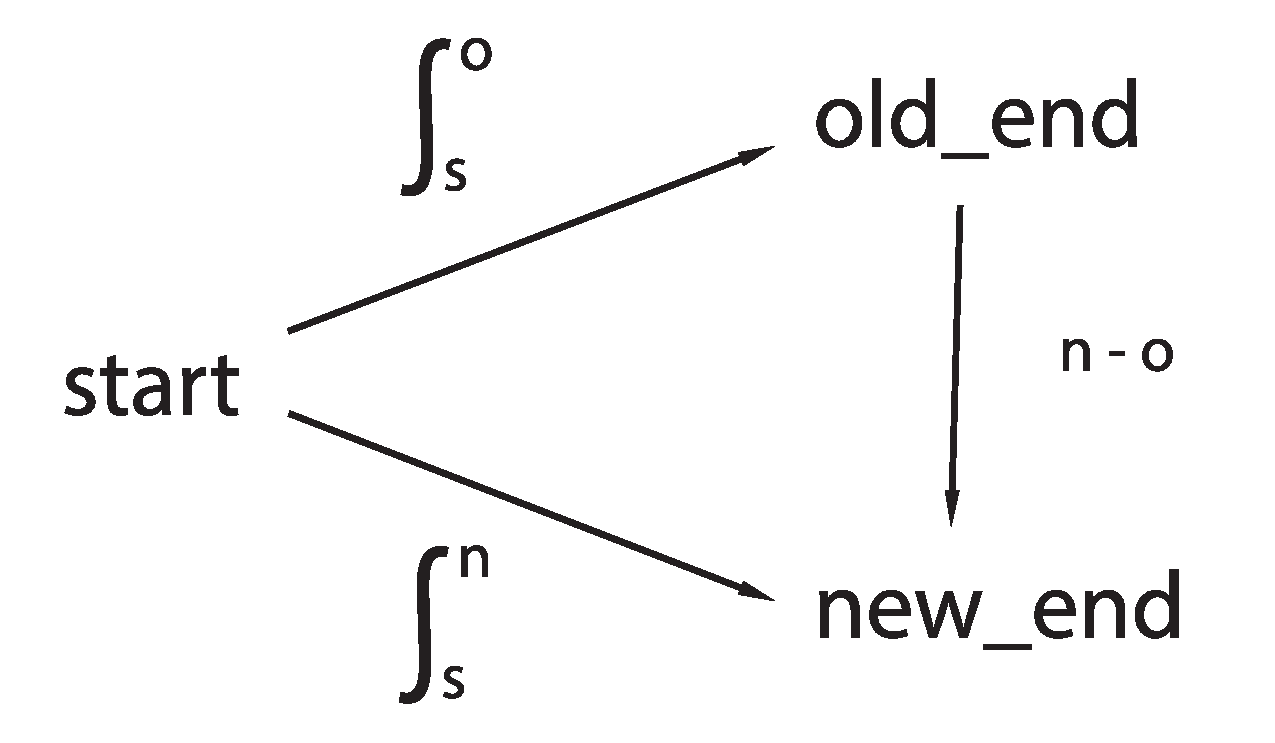
\includegraphics[width=0.95 \linewidth]{isimprovement}
\end{center}

The {\tt start} state is as discussed, {\tt old\_end} is the state at
{\tt now}, and {\tt new\_end} is the state after the potential
improvement sequence. $\int_s^o$ is the integral of score changes
along the {\tt improveme} path and $\int_s^n$ along the candidate
improvement. The integral is the weighted sum of the objectives
increased minus the weighted sum of the objectives that decreased, at
each step, all summed up. This works better than just computing the
weighted score from e.g. {\tt start} to {\tt old\_end} when they are
separated by many frames (typical backtrack distances are several
hundred frames). The expression $n-o$\footnote{This is not numerical
  minus but minus according to the set of objective functions. Just
  roll with it.} is just the weighted sum of objectives that increased
minus the weighted sum of objectives that decreased between the old
end state and new end state; we have no option of computing the
integral here because we don't have an input sequence that goes from
the old end to the new end (and there almost certainly isn't one). We
require that three conditions hold:
\begin{enumerate}
\item $\int_s^n \geq \int_s^o$,
\item $\int_s^n > 0$
\item $n - o > 0$
\end{enumerate}

The integral has to be at least as good as before, the new integral
has to be positive, and the new end state needs to look better than
the old end state (the triangle inequality does not necessarily hold
here). If they all do, then the score for the improvement is $\int_s^n
- \int_s^o + (n - o)$, which is guaranteed to be positive.

Even if we have many possible replacements, we try only the ones with
the best scores; due to the particulars of the implementation there is
not a simple constant describing this maximum, but it's around 220
with the parameter settings used in this paper.

\parameteralert{
  Again! The humiliating appearance of constants! There are many here,
  having to do with the number of potential replacements we use of
  each type, the maximum number we keep, how often we bactrack, and
  how far. I am not totally satisfied with how backtracking works (see
  below), so I don't want to spend too much energy speculating about
  how to reduce the parameter space here; I'd rather replace the
  method wholesale.}

The {\em improvability} of a state is the fraction of these potential
improvements that are legal improvements, as above. Based on my
analysis, states that are highly improvable ($> 30\%$) tend to be
``worse'' (more stuck, closer to death, or whatever) than those that
are not very improvable ($< 5\%$). This isn't being used for anything
currently, but getting an absolute picture of how good a state is (as
opposed to simply comparing it to an adjacent state) is one of the
difficulties with this approach, so this may be a useful notion for
future directions.

\paragraph{Takes of woe, tales of joy.} 
\begin{figure}[h!t!b]
\begin{center}
\includegraphics[width=0.95 \linewidth]{mario13}
\end{center}\vspace{-0.1in}
\caption{After making me feel so successful by finally cleanly
  finishing world {\tt 1-2}, Mario immediately jumps into the first
  trivial pit in {\tt 1-3}. I believe what's going on here is that
  this is actually the best future, because resetting back a single
  screen isn't a large loss, lives aren't included in the objective
  function, and probably the rest of the futures were struggling to
  make progress. This level is very jumpy and probably needs more
  futures to navigate its obstacles. In any case, Mario, Touch\'e.}
\label{fig:mario13}
\end{figure}

Backtracking was initially added in order to fix the mario coin ledge
problem in {\tt 1-2}. It did not help with this. Older versions of the
code would have Mario get past this spot, probably by luck, but in
these he would get stuck in an embarrassing way on a small pit later,
or jump straight into an enemy. Most of the approaches that actually
looked solidly good elsewhere were failing badly here. As I started
writing up this paper, on an airplane, I discovered the bug in the
weighting of objective functions described in
Section~\ref{sec:objectiveweighting}. On my trip I had let {\tt
  playfun} run with particularly high constants ({\tt NFUTURES} = 50,
lots of backtracking candidates, etc.) and it had spent about a
thousand CPU hours playing to this point, grabbing the coins, and then
dying of timeout, then losing all its lives, starting over, and
getting to this point again! After fixing the bug, I tried again, and
it was a huge breakthrough: Mario jumped up to get all the coins, and
then almost immediately jumped back down to continue the level! On his
first try he beat {\tt 1-2} and then immediately jumped in the pit at
the beginning of {\tt 1-3} just as I was starting to feel suuuuuper
smart (Figure~\ref{fig:mario13}). On a scale of OMFG to WTFLOL I was
like {\em whaaaaaaat}?

Seeing this huge improvement changed my idea about what part of the
code needed work (I now believe that simpler search strategies might
work and better lexicographic order generation and weighting is called
for). But, this was already in the midst of writing up the paper, so
instead I spent the CPU time running the current version on a bunch of
games. Those results are described in Section~\ref{sec:results} and
videos are available at \url{http://tom7.org/mario/}. In the next
section I describe some of the performance improvements I made, and
other modifications to the emulator interface.

\section{Performance} \label{sec:performance}

Performance is really important, both because the quality of the
output is CPU-bound and because I am impatient. In its current state,
running {\tt playfun} is an overnight affair; it takes about an hour
of real time to produce 1000 output frames (16 seconds of gameplay) on
a high-end desktop machine. Other than a trick that I didn't end up
using, these performance ideas are not at all new, but they are
documented here for completeness. I certainly spent lots of time on 'em!

\subsection{Caching of emulation} \label{sec:caching}

The most expensive part, by far, is running a step of emulation. It
takes about 500\textmu s to emulate a single frame, though this can
vary depending on what instructions are actually executed (recall that
each frame corresponds to many many 2A03 instructions; there are
approximately 16,000 clock cycles per frame!). Hardware like the
Picture Processing Unit and sound chip are emulated as well, which may
actually be less efficient than the actual hardware (for example, the
sound hardware can implement filtering with passive physical
components like capacitors, but FCEUX contains a finite impulse
response filter running on IEEE floating point numbers). We want to
avoid executing a step more than once, if at all possible.

Caching is so canonical that some have called it (pejoratively) the
only idea in Systems research. And it is what we do here. The emulator
adds a call
%
\begin{code}
void CachingStep(uint8 input);
\end{code}
%
with exactly the same semantics as {\tt Step}. However, it first
checks to see if this exact input has been executed on this exact
start state before. If so, it just restores the cached result
state instead of executing the step.

I use the excellent CityHash function\cite{CityHash} as the hash code,
and use a least-recently-used approach to clean out the hash table
when it has more than a fixed {\em slop} amount more than the target
size. States are large because they contain both the savestate of the
before and after state. I have plenty of RAM, so I allow each process
to store up to 100,000 states with 10,000 states of slop, which takes
about 3 gigabytes per process.

Caching adds a little bit of overhead (a single step is about 13\%
slower, amortized), from saving the state, computing the hash code,
copying the state into the table, and cleaning the hash table
periodically. A cache hit is a zillion times faster than actually
executing the step, however, so as long as the hit rate is more than
13\%, it's worth doing. I use caching step in most places inside {\tt
  playfun}, except when I know that the state can't have been computed
yet. The {\tt playfun algorithm} is particularly suitable to caching:
The set of potential next input sequences {\tt nexts} usually share
several input prefixes, and we keep around futures for some time, so
we can often end up evaluating the same one under the same conditions
many times. Moreover, mutant futures usually share their first half,
making them half price. A really important property of caching is that
it's based on the state of memory but doesn't care about the actual
sequence used to get there. This means that in cases where the input
is ignored (Mario ignores the jump button most of the time while in
the air, for example, and ignores all inputs between levels) we reach
equivalent states and can use the cache if the next input is exactly
the same. The ideal approach here would be to follow how the bits of
the input are actually read by the code, and insert a more generic key
into the hash table. For example, if we see that the code never even
read the bit of the input corresponding to the up direction, then we
can reuse the step for an input that matches all bits but the up bit!
This of course requires a lot of mucking around in the internals,
which on a scale of within the scope to beyond the scope of this
article is a 9.9.

{\bf Software engineering lesson:} Initial results from caching were
disappointing and I thought the overhead was to blame. I made several
low-level tweaks to avoid copying, etc., to reduce the overhead from
36\% to 13\%. Then I discovered that there were 0 cache hits ever,
because of a bug (I was inadvertantly using pointer equality on keys
instead of value equality, so keys were never found). Check basic
things about your code's correctness before going on an optimization
sortie!

\subsection{Space optimizations}

Before I had the idea that is the actual subject of this paper, I was
playing around with other emulator search ideas that involved storing
very very large numbers of states. This necessitated minimal
representations of savestates. FCEUX uses zlib internally to compress
states, which works well; they shrink from something like 13,776
bytes\footnote{I don't completely understand the NES architecture and
  emulation strategy, but I believe some games include expansion chips
  that require more space for save states. All this work is based on
  the 2048 bytes of main NES RAM, as you already know. Perhaps clever
  video game authors from the past can protect against this paper's
  approach by storing important game facts inside expansion chips
  in the cartridge.} to an average of 2266. I made some modifications
to the save/load routines to make this as small as I could manage.
I removed the backing buffer, which is only used for drawing graphics,
movie info, header bytes that are constant or already known (savestate
size), which shrunk the compressed size to an average of 2047.42 bytes.
That meant I could fit about 32 million savestates in RAM at once, which
would be kind of amazing if I could tell my 8 year-old self that.

Compression algoritms work well when there is lots of redundancy in
their input. Comparing memories between two frames in some game,
you'll often see only a few differences. Some of the memory contains
stuff that's essentially read-only, even. To improve the
compressibility of savestates, I introduce the idea of a {\em basis}
state. This is any non-empty sequence of bytes which is an additional
argument to the {\tt LoadState} and {\tt SaveState} functions. It's
subtracted from the savestate prior to compression (it doesn't have to
be the same size; it's treated as an infinite repetition of those
bytes). If the basis is the same as the savestate, then the result is
all zeroes, which compresses nicely (of course, now you need to have
the basis in order to load the state, which is the same as the
savestate, so that didn't save you much!). But memories during
gameplay often don't differ much, so I save a state from any arbitrary
frame in the game and then use that as the basis for everything else.
This factors out any common parts and makes the states much more
compressible: The average size drops to 1870.41 bytes.

Using a better compression algorithm like the Burrows--Wheeler
transform\cite{Burrows}\footnote{This is really one of the all-time
  great algorithms. If you don't know it and you like this kind of
  thing, you should check it out. It's so surprising and elegant.}
would probably help too; zlib implements LZW which is only mediocre.
However, on a scale of throwing my computer out the window to wanting
to reimplement all software in my own private SML library, I just
can't stand getting 3\rd-party libraries to compile and link into my
applications, so I didn't even try. In any case, I abandoned this
direction, which was not working well even with lean savestates.

For {\tt playfun}, RAM is not a bottleneck at all. I disable
compression completely on savestates, including the builtin zlib stuff
(which is actually rather slow) and just use raw savestates. The
removal of unnecessary headers and stuff is still there, and saves a
few bytes and CPU cycles, but there was no reason to actually do it
for this particular work. {\em But sometimes I do unnecessary things.}

\subsection{MARIONET}

The {\tt playfun} algorithm involves running 40 or so different
10-sequence {\tt next} steps and then scoring them against {\tt
  NFUTURES} different futures. Each {\tt next} and each future is
completely independent and dominated by the cost of evaluating
emulator steps. The ideal thing would be to use threads and shared
memory to run these steps in parallel. As I mentioned earlier,
FCEUX is hopelessly single-threaded.

Eventually I realized I needed to search more states than I could in a
single thread, and so I created MARIONET. It's a play on words, a
double entendre of ``Mario network'' and ``Marionette'', which is
obvious. This is a mode whereby {\tt playfun} can be started in
``helper'' mode (listens on a port for work to do) or ``master'' mode
(connects to a list of ports to run work on), in order to run
many emulators in different processes.

The processes communicate over TCP/IP. I only run it on my local
computer, but it would be reasonable to run it on a cluster or
possibly even the Internet. I used SDL's SDL\_Net\cite{SDLNet} as a
portable network interface in the hopes of keeping it
platform-agnostic (FCEUX is basically portable so it would be a shame
to make this Windows-specific, though I am not eager to try to get
this thing to compile on other platforms, I gotta be honest). SDL is a
nightmare to get working with mingw in a 64-bit compile, as usual, and
SDL\_Net contained some bugs\footnote{In particular, the {\tt
    SDLNet\_TCP\_Recv} call is supposed to block until it has received
  the entire requested length, but it occasionally returns early.}
that I had to spend some time working around. Anyway, I'm just
complaining. For serializing requests and responses to bytes, I used
Google's Protocol Buffer library\cite{ProtoBuf}, which is designed for
this kind of thing.

Helpers all start up with the same ROM and motif and objectives
loaded, so that they can simulate whatever the master would
compute.\footnote{Only the master reweights motifs, since it needs a
  single sample of memories that we've observed. That means that in
  cases where a helper generates random motifs, it does so with
  respect to the original human weighting. There are some other small
  things I simply avoided doing because they would require too much
  coordination between processes or make the RPCs too large; MARIONET
  was part of the system for much of its development.} They just wait
on a port for the master to send a request, which can be either ``try
this set of {\tt nexts} with these futures and send me the results'' or
``try to find $n$ improvements of these inputs {\tt improveme} using
so-and-so approach.'' In either case we send the base state as a
serialized savestate.

The master does the outer loop of the algorithm and all the writing to
disk and so on. When it needs to do an expensive step like the inner
loop, it prepares a set of jobs and sends them to workers using a
little fork-join library ({\tt netutil.*}). The library keeps track of
the outstanding jobs and which helpers are working, and feeds them
work when they are idle, until all the jobs are complete. It's even
got a color ANSI progress bar and stuff like that.

Utilization is very good (Figure~\ref{fig:utilization}), and we get
almost a linear speedup with the number of processes, up to the number
of hardware threads the system supports (twelve). Actually, in
addition to the computer remaining usable for other stuff, $n-1$
helpers may work a bit better than $n$, because each of the
helpers is then able to avoid preemption. Since the driver loop is
synchronous, having one laggard process slows the whole darn thing
down while everything waits for it to finish.

\begin{figure}[htb]
\begin{center}
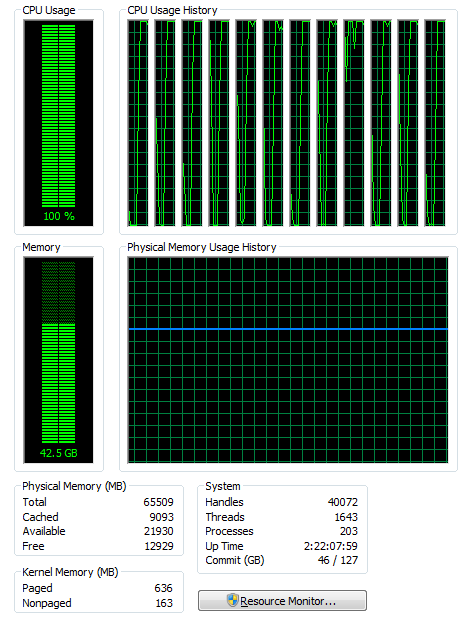
\includegraphics[width=0.75 \linewidth]{utilization}
\end{center}\vspace{-0.1in}
\caption{Utilization with 12 helpers and one master on a 6-core (12
  hyperthreads) processor. Looks good. Keeps the bedroom warm.}
\label{fig:utilization}
\end{figure}

MARIONET is a huge improvement and was what enabled using 40+ futures
in a reasonable amount of time, which is key to high-quality output. It's
obviously the way you want to run the software, if you can get it to
compile. There is one downside, though, which is that it reduces our
ability to get lucky cache hits across {\tt nexts} that are similar (or
have the same effect), and when replaying the winner as we commit to it.
It's worth it, but smartly deciding which helper gets which tasks (because
they share prefixes, for example) would save time. Running it all in one
process with a shared memory cache would be the best, as long as the
lock contention could be kept under control.

\begin{figure}[ht!b]
\begin{center}
\includegraphics[width=0.75 \linewidth]{mario13bug1a} \\[0.3em]
\includegraphics[width=0.75 \linewidth]{mario13bug1b}
\end{center}\vspace{-0.1in}
\caption{Mario bounces off one Goomba up into the feet of another. Not
  only doesn't he have enough velocity to reach the platform, but he's
  about to hit that Goomba from below. Believe it or not, this ends
  well: {\tt playfun} is happy to exploit bugs in the game; in this case,
  that whenever Mario is moving downward (his jump crests just before the
  Goomba hits him) this counts as ``stomping'' on an enemy, even if that
  enemy is above him. The additional bounce from this Goomba also allows
  him to make it up to the platform, which he wouldn't have otherwise!
}
\label{fig:mario13bug1}
\end{figure}

\section{Results} \label{sec:results}

In this section I describe the results of running {\tt learnfun} and
{\tt playfun} on several NES games. These games were all played with
the same settings developed and tuned for Super Mario Bros.; that is,
this was the result of just running the program the first time on a
recording of me playing the game briefly. Every game I tried is
documented here; lack of CPU time before conference is the main reason
your favorite is not included. The website \url{http://tom7.org/mario/}
contains video versions of some of these, which may be more fun. Let's
begin with the {\em ur} game, Super Mario Bros..

\subsection{Super Mario Bros.}

This game is an obvious benchmark and the one I used during the
development of {\tt learnfun} and {\tt playfun}. Some parts of the
algorithm (see e.g. Section~\ref{sec:backtracking}) were developed
specifically to get around problems in the ability to play this game,
though I believe simpler methods would also work on this game, now
that some important bugs are fixed.

Automated Mario is fun to watch, and definitely my favorite. The
familiarity of the game, the combination of human-like maneuvers and
completely bizarre stuff, daredevil play, and bug exploitation
(Figure~\ref{fig:mario13bug1}) are all a delight. It's even funny when
it fails, watching Mario struggling with obstacles like tiny pits, or
making a heroic move followed by a trivial mistake. I recommend
watching the videos.

This algorithm works well on Super Mario Bros., and I think that with
some improvements it could play quite far into the game. It probably
can't beat the game; Worlds {\tt 7-4} and {\tt 8-4} require some weird
puzzling that we all needed {\em Nintendo Power Magazine}'s help to
solve as kids, and are not just a matter of running to the right and
avoiding obstacles. In the current incarnation, Mario breezes through
World {\tt 1-1} every time, consistently beats {\tt 1-2} (I've only
tried about three times with the newest version of the code, but each
time he's succeeded) and has limited success on {\tt 1-3} but
eventually suicides too many times. I'll keep trying.

The Mortal Kombat-style {\em Finish Him!} to any machine learning
algorithm is overfitting, however. Does the technique work on other
games, without endless tweaking as I did with Super Mario Bros.? On a
scale of no to yes, this is both a 1 and a 10; some games work even
better than Mario and some are a disaster.

\subsection{Hudson's Adventure Island}

This is a bad, difficult, but likable game featuring a skateboarding
cherubic island guy called Master Higgins, whose girlfriend has been
kidnapped by King Quiller. He basically runs to the right and can
throw or ride stuff that he finds in eggs. The controls are pretty
soft and danger is everywhere. The objective functions that work are
probably pretty similar to Super Mario Bros., but there are fewer
obstacles to navigate---the difficulty for humans mostly comes from
the speed and reaction time. Master Higgins doesn't care about bumping
into rocks and dropping his health almost to nothing (but then is
careful about health), and once he gets a weapon his aim anticipates
off-screen enemies and he looks pretty savvy
(Figure~\ref{fig:adventureisland}). His weakness regards holes in the
ground, which he sometimes jumps into, probably for the same reason
that Mario sometimes does. His ``pot bonus'' was 16720. Master Higgins
beats several levels and makes it into the cave before losing his last
life by jumping straight into a vibrating skull with swirling
fireballs around it, which on a scale of Darwin Award to dignified
demise is approximately a 6, in my opinion.

\begin{figure}[ht]
\begin{center}
\includegraphics[width=0.95 \linewidth]{adventureisland}
\end{center}\vspace{-0.1in}
\caption{Master Higgins putting safety first.}
\label{fig:adventureisland}
\end{figure}

\subsection{Pac-Man}

One of the smallest NES games at a mere 24kb, Pac-Man is a classic
that I won't belabor. It has a fairly straightforward objective---your
score---and there is no timer or anything to worry about but the
ghosts. A good planner could probably solve Pac-Man with just score as
an objective (keep in mind that with RAM inspection and because of
ghost movement, this is not just a simple matter of using A$^{*}$ or
something to plan a path through the Euclidean grid---states aren't
repeated hardly ever). Automating this game works pretty well; Pac-Man
doesn't have much trouble avoiding ghosts except when they trap him.
Play is pretty strange: He doesn't necessarily grab nearby dots (hard
to explain) and often switches direction in the middle of a corridor,
unlike human play which is usually efficient sweeps of the dots when
ghosts aren't near. However, automating has a huge advantage over
human players with respect to ghosts, and Pac-Man is alarmingly
fearless. He chases ghosts down corridors, turns straight into them,
knowing that they will change direction in time to not run into him
(this makes the time travel advantage quite stark).
Figure~\ref{fig:pacman} shows gratuitous daredeviling as he ducks in
and out of a tiny sliver of space between two ghosts, then does it
again, and survives.

Eventually, Pac-Man gets far enough away from the remaining dots that
none of his futures bring him near, and without any other objective
to seek out, runs into ghosts. He dies on the first level with 13 dots
left.

\begin{figure}[h!t!]
\begin{center}
\includegraphics[width=0.75 \linewidth]{pacman1} \\[0.3em]
\includegraphics[width=0.75 \linewidth]{pacman2} \\[0.3em]
\includegraphics[width=0.75 \linewidth]{pacman3}
\end{center}\vspace{-0.1in}
\caption{Pac-Man showing utter disregard for the ghosts's personal
  space. This occurs around frame 6700 of the output movie. Pac-Man
  slips into the space between Blinky and Inky to touch the wall,
  comes out unharmed, then momentarily teases Clyde before escaping
  to vibrate some more in empty corridors.}
\label{fig:pacman}
\end{figure}

\subsection{Karate Kid, The} \label{sec:karate}

\begin{figure}[htb]
\begin{center}
\includegraphics[width=0.95 \linewidth]{karate}
\end{center}\vspace{-0.1in}
\caption{
  Daniel-San blowing his last Crane Kick on a karate noob like there's
  no tomorrow, which there won't be if he uses up all his power moves
  like that. Note that the {\bf Chop} approach to backtracking was
  used to generate this movie frame, appropriately.}
\label{fig:karate}
\end{figure}

Karate Kid, The, is the typical trainwreck that follows when a beloved
movie is turned into a video game. The game has awful controls and
integer-only physics with massive throw-back upon collision, strange
mini-games with no explanation, annoying debris flying through the
sky, and luck-based fighting. It was probably only ever finished by
kids with extreme discipline and self-loathing, or kids with only one
video game available to them. It begins with a karate tournament which
is even less fun than the main game, which is sort of a platformer
with very few platforms.

In this game I played 1,644 frames, just the first two of four
opponents in the karate tournament. Automated by {\tt playfun}
Daniel-San is able to punch and kick the low-level karate noobs,
preferring to spend all his super-strong Crane Kick power moves right
away. His style doesn't make much sense, sometimes facing away from
the opponent, or throwing punches and kicks when the opponent isn't
near. He doesn't worry much about taking damage. He gets to the final
round and makes a valiant effort, at one point taking himself and the
karate boss to 0 health simultaneously. But in this game, tie goes to
the computer-controlled player without feelings, so it's back to the
title screen for Daniel-San. The result is not impressive at all; the
main goal here is to reduce the opponent's health, but our objective
function can only track bytes that go {\em up}. Still, the automated
version gets farther than my input did.

\subsection{Bubble Bobble} \label{sec:bubblebobble}

Let's take a journey to the cave of monsters! This lovely game
features two stout dinosaurs called Bub and Bob, who jump around in a
series of single-screen caves. You can shoot bubbles to encase
monsters and then pop the bubble to turn them into fruit or other
treasure; clearing all the monsters takes you to the next stage.
Bubbles are also necessary for navigating around, since you can bounce
on your own bubbles when holding the jump button.

I was surprised that automating this game works at all, since there is
no obvious spatial gradient like in Super Mario Bros., and few local
greedy rewards like in Pac-Man. Bub initially wastes his lives (a
common theme in games where the respawn interval is low---it just
looks like a fast way of warping to the corner). When he's near
monsters he shows good tactics in shooting and popping them
simultaneously, even doing so while facing away from them, which I
didn't know was possible. At the beginning of the movie he prefers to
hide in the bottom-left corner, but soon starts jumping all around the
level, bouncing on his own bubbles and so on, almost like a real
player would. He beats more levels than my input movie did! Since it
takes two start button presses to enter the game, the second START is
part of the input motifs. Amusingly, Bub uses this to his advantage to
change the synchronization of his futures, and when the situation gets
really tight, he'll pause the game until a good future comes around
(Figure~\ref{fig:bubblebobble}). Paused states probably look like
modest progress since memory locations like the music cursor are still
advancing.

After a harrowing escape from the ghost thing on level 4, Bub makes it
to level 5 (my input movie quits at the beginning of level 4!), at
which point I stopped the search because it was getting pretty pausey
and I wanted to see some other games before the SIGBOVIK deadline.

\begin{figure}[ht]
\begin{center}
\includegraphics[width=0.95 \linewidth]{bubblebobble}
\end{center}\vspace{-0.1in}
\caption{Bub navigates this game surprisingly well. Once he's on his
  last life, he becomes careful and pauses the game when things are
  looking grim---here pausing for about a thousand frames, burning
  through the futures until one randomly comes along that looks good.
  He then unpauses and executes that good future, killing three of
  these monsters in short order.}
\label{fig:bubblebobble}
\end{figure}

\subsection{Color a Dinosaur}

\begin{figure}[ht]
\begin{center}
\includegraphics[width=0.95 \linewidth]{dinosaur}
\end{center}\vspace{-0.1in}
\caption{The second dinosaur colored by the {\tt playfun} algorithm.
  There's no way to go wrong in this game; any possible coloring is
  {\em oh so right}.}
\label{fig:dinosaur}
\end{figure}

This is a strange NES ``game'' where you do the eponymous action,
probably intended for kids. It's not very fun to watch the weird slow
floodfill algorithm color in parts of a dinosaur, and there's no
objective to be found. Predictably, the approach of this paper doesn't
simulate human play very well. There doesn't even seem to be an
objective for humans to suss out, except for the open-world sandbox of
two-color dinosaur coloring. The automated pencil manages to ``color''
two different dinosaurs (Figure~\ref{fig:dinosaur}), though the play
looks pretty spastic and random.

\subsection{Tetris}

\begin{figure}[ht]
\begin{center}
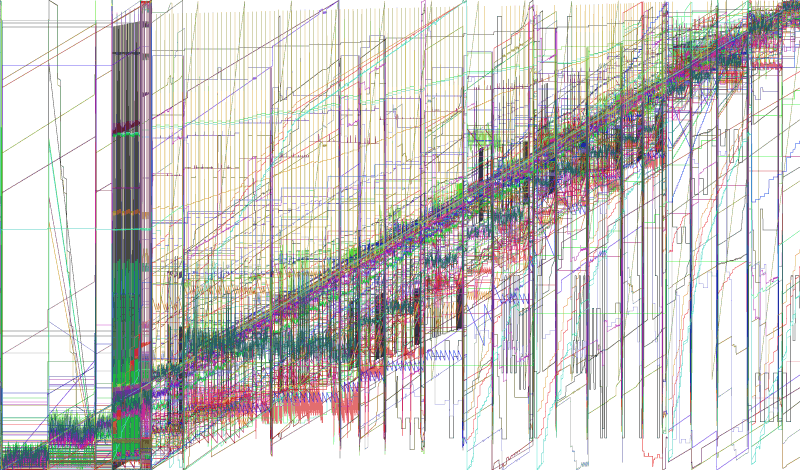
\includegraphics[width=0.95 \linewidth]{tetris}
\end{center}\vspace{-0.1in}
\caption{The joyful noise of objective functions learned for Tetris.
  The first fifth of the movie is navigating menus and looks very
  different from the remainder. There appear to be some frame counters
  identified, which make perfect smooth progress throughout the entire
  movie. I believe discontinuities correspond to placing of pieces;
  some objectives monotonically increase at these points (and are noisy
  in-between), suggesting that they incorporate the score.
}
\label{fig:tetris-objectives}
\end{figure}

\begin{figure}[ht]
\begin{center}
\includegraphics[width=0.95 \linewidth]{tetris-tower}
\end{center}\vspace{-0.1in}
\caption{Would you hire this construction company? Death is imminent,
so {\tt playfun} pauses the game shortly after this and then doesn't
unpause it.}
\label{fig:tetris-tower}
\end{figure}

Tetris is a block dropping game, also known to the ancients. The
Nintendo implementation is infamous for being inferior to the
unlicensed Tengen version, which Nintendo tried to sue out of
existence. Here I try to automate the Nintendo version as a tribute to
litigation. Unsurprisingly, {\tt playfun} is awful at this game.
Tetris has several screens of menus, where the player can select
between different modes and theme musics and stuff like that. As an
amusing prelude to this disaster in tetromino stacking, {\tt playfun}
keeps entering the menu and exiting back to the title screen rapidly,
taking several seconds to even start the game. (Like in Bubble Bobble,
this means that the start button is among the motifs.) Although the
piece dropping looks more or less natural (but it's hard to not be, as
the game drops the pieces for you), the placement is idiotic---worse
than random. This may be because placing a piece gives you a small
amount of points, which probably looks like progress
(Figure~\ref{fig:tetris-objectives}), so there is incentive to stack
the pieces as soon as possible rather than pack them in. As the screen
fills, there's a tiny amount of tetris-like gameplay, probably as the
end of the game becomes visible in some of the futures. The end result
is awful and {\tt playfun} makes zero lines and certainly no Tetrises
(Figure~\ref{fig:tetris-tower}). The only cleverness is pausing the
game right before the next piece causes the game to be over, and
leaving it paused. Truly, the only winning move is not to play.

\section{Future Work}

It is famous last words, but I actually intend to keep working on this
project. Because of SIGBOVIK crunch pressure (and discovering some
bugs as I was writing the paper) the approach got much better very
recently and I'm mostly limited by CPU hours until conference. It's
today in a state where whenever I run it on a new game I see something
delightful. Even just running it on more of the NES classics is
worthwhile. However, I have lots of ideas about how to extend the
technique, either to make it more beautiful or to make it work better:

\paragraph{Parameter reduction.}
I've already pointed out the places where there are mysterious
constants in the code. Although the fact that the same constants work
on many different games without tuning is some solace, it would really
be nicer to remove these. One of the hardest to remove is the length
of the futures explored. And I like a challenge!

\paragraph{Unsupervised learning.}
Speaking of challenge, it might be possible for {\tt playfun} to teach
itself, by starting with no objective functions and playing randomly
to see what bytes it {\em can} make go up, then fitting lexicographic
orderings to the memories and repeating. The beginnings of games
(which include RAM intialization, title screens, and menus) continue
to vex this kind of work, unfortunately.

\paragraph{Generalized orderings.}
Right now, lexicographic orderings are limited to vectors of unsigned
bytes that get larger. Many games treat bytes as signed (I believe
this is true of Mario's velocity, for example). For other bytes, like
one representing your enemy's health (c.f. Karate Kid), winning means
making the byte {\em go down}, not up. It is possible to generalize
the lexicographic orderings we generate to a vector of ($L_i$, $<_i$)
pairs, where $<_i$ tells us how to compare the bytes at that location.
Things to try would be two's-complement signed comparison, or unsigned
greater-than. I think this is a great avenue; the dangers are
overfitting (now most short sequences can be explained in one way or
another) and being too fancy.

\paragraph{Input models.}
I'm unsatisfied with the motif approach. As mentioned earlier, the
obvious thing to try instead is a Markov model, which would probably
be simpler and would allow re-weighting from inputs regardless of what
we concocted while playing (the current version can only reweight the
human motifs, not learn new sequences discovered while running). I
would also like some solution to the start button problem---if it is
among the motifs, it often shows up in gameplay in annoying ways. I
don't feel good about simply blacklisting it, however. In Bubble
Bobble, start appears to be used to burn away futures when all of them
are bad. Maybe a simple improvement would be to allow the inner loop
of {\tt playfun} to skip the turn (empty {\tt next} sequence) in
order to simulate this.

\paragraph{Better backtracking.}
Backtracking is a powerful idea, and there's lots more to do here. The
fixed-size backtracking window is disappointing since it's a
parameter, and doesn't even seem right for most games. It would make
sense to do something like lengthen the window until the {\em
  improvability} starts dropping; basically, find the amount of recent
past that's comparable to random play, and try improving that.
Moreover, it should be possible to re-backtrack, since some parts of
the game are harder than others. Ideally, when Mario has so few
options that he contemplates suicide, he should be backtracking over
and over and farther and farther until he finds a future that's good.
This is the power of time travel. Use it, man.

\paragraph{Efficiency in search}
Quality is directly related to the number of states searched. Some
sequences are easier to search than others, because they share a prefix
with something we've already done and can be cached. It would be worth
looking into algorithms that explicitly take into account the cost of
branching, so that we explore some tree (of futures, for example) rather
than disjoint linear futures. The effective number of futures explored
could be much higher for the same CPU.

\paragraph{Multiple players, multiple games.}
Other than the particulars of the way it's built (\verb+vector<uint8>+
everywhere), there's no reason why the technique is limited to a
single player's input. In a game like Bubble Bobble or Contra the two
players can collaborate in interesting ways, and planning both
simultaneously would probably lead to occasional awesome results. For
example, in Contra, it might be that one player is shooting enemies
for the other player, the bullets arriving from across the screen just
in time to save him as he blithely jumps into danger. Another clever
feat from the Tool Assisted Speedrun community is a sequence of inputs
that beats multiple different {\em games} simultaneously. For example,
human geniuses used tools to beat Mega Man (Mega Men?) 3, 4, 5, and 6
all at the same time using the exact same input sequence sent to all
four games.\cite{BaxterTAS} I think the algorithms in this paper apply
directly---it's just a matter of multiplexing the inputs to each of
the games, and then taking the appropriate operation (min, max, sum)
of their objective functions to produce a final objective function.
The main obstacle is the architecture of the underlying emulator,
which can only load one game into its global variables at once.

\section{Conclusion}

In this paper I showed how lexicographic orderings and time travel can
be used to automate classic video games. The approach uses an
amusingly simple and mathematically elegant model to learn what
constitutes ``winning'' according to a human player's inputs. It then
uses hundreds of CPU hours to search different input sequences that
seem to ``win'', inspecting only the RAM of the simulated game,
ignoring any of the human outputs like video and sound. The technique
works great on some games, getting farther into the game than the
human's inputs did, and produces novel gameplay (for example, bug
exploitation and super-human daredevil timing). On other games, it is
garbage, but on a scale of recycling symbol 1 to recycling symbol 7,
it is at least hilarious garbage.

\bibliographystyle{plain}
% \bibliographycomment{} % nothing
\bibliography{paper}

\end{document}
